% Options for packages loaded elsewhere
\PassOptionsToPackage{unicode}{hyperref}
\PassOptionsToPackage{hyphens}{url}
\documentclass[
  man, donotrepeattitle]{apa6}
\usepackage{xcolor}
\usepackage{amsmath,amssymb}
\setcounter{secnumdepth}{-\maxdimen} % remove section numbering
\usepackage{iftex}
\ifPDFTeX
  \usepackage[T1]{fontenc}
  \usepackage[utf8]{inputenc}
  \usepackage{textcomp} % provide euro and other symbols
\else % if luatex or xetex
  \usepackage{unicode-math} % this also loads fontspec
  \defaultfontfeatures{Scale=MatchLowercase}
  \defaultfontfeatures[\rmfamily]{Ligatures=TeX,Scale=1}
\fi
\usepackage{lmodern}
\ifPDFTeX\else
  % xetex/luatex font selection
\fi
% Use upquote if available, for straight quotes in verbatim environments
\IfFileExists{upquote.sty}{\usepackage{upquote}}{}
\IfFileExists{microtype.sty}{% use microtype if available
  \usepackage[]{microtype}
  \UseMicrotypeSet[protrusion]{basicmath} % disable protrusion for tt fonts
}{}
\makeatletter
\@ifundefined{KOMAClassName}{% if non-KOMA class
  \IfFileExists{parskip.sty}{%
    \usepackage{parskip}
  }{% else
    \setlength{\parindent}{0pt}
    \setlength{\parskip}{6pt plus 2pt minus 1pt}}
}{% if KOMA class
  \KOMAoptions{parskip=half}}
\makeatother
% Make \paragraph and \subparagraph free-standing
\makeatletter
\ifx\paragraph\undefined\else
  \let\oldparagraph\paragraph
  \renewcommand{\paragraph}{
    \@ifstar
      \xxxParagraphStar
      \xxxParagraphNoStar
  }
  \newcommand{\xxxParagraphStar}[1]{\oldparagraph*{#1}\mbox{}}
  \newcommand{\xxxParagraphNoStar}[1]{\oldparagraph{#1}\mbox{}}
\fi
\ifx\subparagraph\undefined\else
  \let\oldsubparagraph\subparagraph
  \renewcommand{\subparagraph}{
    \@ifstar
      \xxxSubParagraphStar
      \xxxSubParagraphNoStar
  }
  \newcommand{\xxxSubParagraphStar}[1]{\oldsubparagraph*{#1}\mbox{}}
  \newcommand{\xxxSubParagraphNoStar}[1]{\oldsubparagraph{#1}\mbox{}}
\fi
\makeatother
\usepackage{color}
\usepackage{fancyvrb}
\newcommand{\VerbBar}{|}
\newcommand{\VERB}{\Verb[commandchars=\\\{\}]}
\DefineVerbatimEnvironment{Highlighting}{Verbatim}{commandchars=\\\{\}}
% Add ',fontsize=\small' for more characters per line
\usepackage{framed}
\definecolor{shadecolor}{RGB}{248,248,248}
\newenvironment{Shaded}{\begin{snugshade}}{\end{snugshade}}
\newcommand{\AlertTok}[1]{\textcolor[rgb]{0.94,0.16,0.16}{#1}}
\newcommand{\AnnotationTok}[1]{\textcolor[rgb]{0.56,0.35,0.01}{\textbf{\textit{#1}}}}
\newcommand{\AttributeTok}[1]{\textcolor[rgb]{0.13,0.29,0.53}{#1}}
\newcommand{\BaseNTok}[1]{\textcolor[rgb]{0.00,0.00,0.81}{#1}}
\newcommand{\BuiltInTok}[1]{#1}
\newcommand{\CharTok}[1]{\textcolor[rgb]{0.31,0.60,0.02}{#1}}
\newcommand{\CommentTok}[1]{\textcolor[rgb]{0.56,0.35,0.01}{\textit{#1}}}
\newcommand{\CommentVarTok}[1]{\textcolor[rgb]{0.56,0.35,0.01}{\textbf{\textit{#1}}}}
\newcommand{\ConstantTok}[1]{\textcolor[rgb]{0.56,0.35,0.01}{#1}}
\newcommand{\ControlFlowTok}[1]{\textcolor[rgb]{0.13,0.29,0.53}{\textbf{#1}}}
\newcommand{\DataTypeTok}[1]{\textcolor[rgb]{0.13,0.29,0.53}{#1}}
\newcommand{\DecValTok}[1]{\textcolor[rgb]{0.00,0.00,0.81}{#1}}
\newcommand{\DocumentationTok}[1]{\textcolor[rgb]{0.56,0.35,0.01}{\textbf{\textit{#1}}}}
\newcommand{\ErrorTok}[1]{\textcolor[rgb]{0.64,0.00,0.00}{\textbf{#1}}}
\newcommand{\ExtensionTok}[1]{#1}
\newcommand{\FloatTok}[1]{\textcolor[rgb]{0.00,0.00,0.81}{#1}}
\newcommand{\FunctionTok}[1]{\textcolor[rgb]{0.13,0.29,0.53}{\textbf{#1}}}
\newcommand{\ImportTok}[1]{#1}
\newcommand{\InformationTok}[1]{\textcolor[rgb]{0.56,0.35,0.01}{\textbf{\textit{#1}}}}
\newcommand{\KeywordTok}[1]{\textcolor[rgb]{0.13,0.29,0.53}{\textbf{#1}}}
\newcommand{\NormalTok}[1]{#1}
\newcommand{\OperatorTok}[1]{\textcolor[rgb]{0.81,0.36,0.00}{\textbf{#1}}}
\newcommand{\OtherTok}[1]{\textcolor[rgb]{0.56,0.35,0.01}{#1}}
\newcommand{\PreprocessorTok}[1]{\textcolor[rgb]{0.56,0.35,0.01}{\textit{#1}}}
\newcommand{\RegionMarkerTok}[1]{#1}
\newcommand{\SpecialCharTok}[1]{\textcolor[rgb]{0.81,0.36,0.00}{\textbf{#1}}}
\newcommand{\SpecialStringTok}[1]{\textcolor[rgb]{0.31,0.60,0.02}{#1}}
\newcommand{\StringTok}[1]{\textcolor[rgb]{0.31,0.60,0.02}{#1}}
\newcommand{\VariableTok}[1]{\textcolor[rgb]{0.00,0.00,0.00}{#1}}
\newcommand{\VerbatimStringTok}[1]{\textcolor[rgb]{0.31,0.60,0.02}{#1}}
\newcommand{\WarningTok}[1]{\textcolor[rgb]{0.56,0.35,0.01}{\textbf{\textit{#1}}}}
\usepackage{graphicx}
\makeatletter
\newsavebox\pandoc@box
\newcommand*\pandocbounded[1]{% scales image to fit in text height/width
  \sbox\pandoc@box{#1}%
  \Gscale@div\@tempa{\textheight}{\dimexpr\ht\pandoc@box+\dp\pandoc@box\relax}%
  \Gscale@div\@tempb{\linewidth}{\wd\pandoc@box}%
  \ifdim\@tempb\p@<\@tempa\p@\let\@tempa\@tempb\fi% select the smaller of both
  \ifdim\@tempa\p@<\p@\scalebox{\@tempa}{\usebox\pandoc@box}%
  \else\usebox{\pandoc@box}%
  \fi%
}
% Set default figure placement to htbp
\def\fps@figure{htbp}
\makeatother
% definitions for citeproc citations
\NewDocumentCommand\citeproctext{}{}
\NewDocumentCommand\citeproc{mm}{%
  \begingroup\def\citeproctext{#2}\cite{#1}\endgroup}
\makeatletter
 % allow citations to break across lines
 \let\@cite@ofmt\@firstofone
 % avoid brackets around text for \cite:
 \def\@biblabel#1{}
 \def\@cite#1#2{{#1\if@tempswa , #2\fi}}
\makeatother
\newlength{\cslhangindent}
\setlength{\cslhangindent}{1.5em}
\newlength{\csllabelwidth}
\setlength{\csllabelwidth}{3em}
\newenvironment{CSLReferences}[2] % #1 hanging-indent, #2 entry-spacing
 {\begin{list}{}{%
  \setlength{\itemindent}{0pt}
  \setlength{\leftmargin}{0pt}
  \setlength{\parsep}{0pt}
  % turn on hanging indent if param 1 is 1
  \ifodd #1
   \setlength{\leftmargin}{\cslhangindent}
   \setlength{\itemindent}{-1\cslhangindent}
  \fi
  % set entry spacing
  \setlength{\itemsep}{#2\baselineskip}}}
 {\end{list}}
\usepackage{calc}
\newcommand{\CSLBlock}[1]{\hfill\break\parbox[t]{\linewidth}{\strut\ignorespaces#1\strut}}
\newcommand{\CSLLeftMargin}[1]{\parbox[t]{\csllabelwidth}{\strut#1\strut}}
\newcommand{\CSLRightInline}[1]{\parbox[t]{\linewidth - \csllabelwidth}{\strut#1\strut}}
\newcommand{\CSLIndent}[1]{\hspace{\cslhangindent}#1}
\ifLuaTeX
\usepackage[bidi=basic]{babel}
\else
\usepackage[bidi=default]{babel}
\fi
\babelprovide[main,import]{english}
% get rid of language-specific shorthands (see #6817):
\let\LanguageShortHands\languageshorthands
\def\languageshorthands#1{}
\ifLuaTeX
  \usepackage[english]{selnolig} % disable illegal ligatures
\fi
\setlength{\emergencystretch}{3em} % prevent overfull lines
\providecommand{\tightlist}{%
  \setlength{\itemsep}{0pt}\setlength{\parskip}{0pt}}
% Manuscript styling
\usepackage{upgreek}
\captionsetup{font=singlespacing,justification=justified}

% Table formatting
\usepackage{longtable}
\usepackage{lscape}
% \usepackage[counterclockwise]{rotating}   % Landscape page setup for large tables
\usepackage{multirow}		% Table styling
\usepackage{tabularx}		% Control Column width
\usepackage[flushleft]{threeparttable}	% Allows for three part tables with a specified notes section
\usepackage{threeparttablex}            % Lets threeparttable work with longtable

% Create new environments so endfloat can handle them
% \newenvironment{ltable}
%   {\begin{landscape}\centering\begin{threeparttable}}
%   {\end{threeparttable}\end{landscape}}
\newenvironment{lltable}{\begin{landscape}\centering\begin{ThreePartTable}}{\end{ThreePartTable}\end{landscape}}

% Enables adjusting longtable caption width to table width
% Solution found at http://golatex.de/longtable-mit-caption-so-breit-wie-die-tabelle-t15767.html
\makeatletter
\newcommand\LastLTentrywidth{1em}
\newlength\longtablewidth
\setlength{\longtablewidth}{1in}
\newcommand{\getlongtablewidth}{\begingroup \ifcsname LT@\roman{LT@tables}\endcsname \global\longtablewidth=0pt \renewcommand{\LT@entry}[2]{\global\advance\longtablewidth by ##2\relax\gdef\LastLTentrywidth{##2}}\@nameuse{LT@\roman{LT@tables}} \fi \endgroup}

% \setlength{\parindent}{0.5in}
% \setlength{\parskip}{0pt plus 0pt minus 0pt}

% Overwrite redefinition of paragraph and subparagraph by the default LaTeX template
% See https://github.com/crsh/papaja/issues/292
\makeatletter
\renewcommand{\paragraph}{\@startsection{paragraph}{4}{\parindent}%
  {0\baselineskip \@plus 0.2ex \@minus 0.2ex}%
  {-1em}%
  {\normalfont\normalsize\bfseries\itshape\typesectitle}}

\renewcommand{\subparagraph}[1]{\@startsection{subparagraph}{5}{1em}%
  {0\baselineskip \@plus 0.2ex \@minus 0.2ex}%
  {-\z@\relax}%
  {\normalfont\normalsize\itshape\hspace{\parindent}{#1}\textit{\addperi}}{\relax}}
\makeatother

\makeatletter
\usepackage{etoolbox}
\patchcmd{\maketitle}
  {\section{\normalfont\normalsize\abstractname}}
  {\section*{\normalfont\normalsize\abstractname}}
  {}{\typeout{Failed to patch abstract.}}
\patchcmd{\maketitle}
  {\section{\protect\normalfont{\@title}}}
  {\section*{\protect\normalfont{\@title}}}
  {}{\typeout{Failed to patch title.}}
\makeatother

\usepackage{xpatch}
\makeatletter
\xapptocmd\appendix
  {\xapptocmd\section
    {\addcontentsline{toc}{section}{\appendixname\ifoneappendix\else~\theappendix\fi: #1}}
    {}{\InnerPatchFailed}%
  }
{}{\PatchFailed}
\makeatother
\keywords{keywords\newline\indent Word count: 4437}
\DeclareDelayedFloatFlavor{ThreePartTable}{table}
\DeclareDelayedFloatFlavor{lltable}{table}
\DeclareDelayedFloatFlavor*{longtable}{table}
\makeatletter
\renewcommand{\efloat@iwrite}[1]{\immediate\expandafter\protected@write\csname efloat@post#1\endcsname{}}
\makeatother
\usepackage{lineno}

\linenumbers
\usepackage{csquotes}
\raggedbottom
\usepackage{endfloat}
\usepackage{setspace}\doublespacing
\usepackage{lineno}
\linenumbers
\usepackage{tabu}
\usepackage{pdflscape}
\newcommand{\blandscape}{\begin{landscape}}
\newcommand{\elandscape}{\end{landscape}}
\usepackage{sectsty}\allsectionsfont{\raggedright}
\usepackage{bookmark}
\IfFileExists{xurl.sty}{\usepackage{xurl}}{} % add URL line breaks if available
\urlstyle{same}
\hypersetup{
  pdftitle={Effect of experimental habitat connectivity on dung beetle communities},
  pdfauthor={Eric Escobar-Chena1, Julian Resasco2, \& Emilio M. Bruna1,3},
  pdflang={en-EN},
  pdfkeywords={keywords},
  hidelinks,
  pdfcreator={LaTeX via pandoc}}

\title{Effect of experimental habitat connectivity on dung beetle communities}
\author{Eric Escobar-Chena\textsuperscript{1}, Julian Resasco\textsuperscript{2}, \& Emilio M. Bruna\textsuperscript{1,3}}
\date{}


\shorttitle{dung beetles and habitat corridors}

\authornote{

We thank the USDA Forest Service for maintaining experimental landscapes and assisting in getting established at the site. We also wanted to specifically thank Thomas Smith for his help in data collection, Sara Escobar-Chena for her help in processing and data entry. Funding was provided by -----.

The authors made the following contributions. Eric Escobar-Chena: Conceptualization, Methodology, Investigation, Formal analysis, Data curation, Software, Visualization, Writing - Original Draft Preparation, Writing - Review \& Editing; Julian Resasco: Conceptualization, Methodology, Writing - Original Draft Preparation, Writing - Review \& Editing; Emilio M. Bruna: Conceptualization, Methodology, Investigation, Formal analysis, Data curation, Visualization, Writing - Original Draft Preparation, Writing - Review \& Editing, Project administration, Supervision.

Correspondence concerning this article should be addressed to Eric Escobar-Chena, University of Florida. E-mail: \href{mailto:eescobarchena@ufl.edu}{\nolinkurl{eescobarchena@ufl.edu}}

}

\affiliation{\vspace{0.5cm}\textsuperscript{1} Department of Wildlife Ecology \& Conservation, University of Florida, PO Box 110530, Gainesville, Florida, 32611-0430 USA\\\textsuperscript{2} University of Colorado, Boulder\\\textsuperscript{3} Center for Latin American Studies, University of Florida, PO Box 110530, Gainesville, Florida, 32611-0530 USA}

\note{

A preprint of this article has been posted at ----- Preprints (link).

ORCID:
EEC: ---- \textbar{}
EB: 0000-0003-3381-8477 \textbar{}
JR: ----- \textbar{}

\newpage

}

\abstract{%
Habitat fragmentation threatens biodiversity across the globe as habitat loss, isolation, and edge effects become increasingly prevalent. Corridors have become an important tool in order to combat the negative effects of fragmentation, however they are difficult to study in natural systems without incurring confounding effects. To observe changes in insect community composition as an effect of landscape features we sampled dung beetles in a landscape scale experiment. We did not see a difference in species richness or diversity, but dung beetle abundances were higher in continuous forest habitat and open habitat patches connected by a corridors than in isolated patches.
}



\begin{document}
\maketitle

\subsection{INTRODUCTION}\label{introduction}

As human disturbances continue to expand into natural landscapes, intact habitats are becoming increasingly fragmented (Taubert et al. 2018, Díaz et al. 2019, Ma et al. 2023). Like many ecological processes, fragmentation is a complex and multifaceted phenomenon bringing about many consequences which can be both positive and negative for ecosystems (Fahrig 2003, Fletcher et al. 2018). However, as habitats are broken down community structures are significantly altered (Harrison and Bruna 1999, Haddad et al. 2003, Jennings and Tallamy 2006, Laurance et al. 2018). This alteration of structure typically lends to loss in biodiversity on a global scale and interruptions in ecosystem processes and functions (Haddad 2015).

Corridors have been shown to be an important mechanism for for minimizing negative consequences of fragmentation (Haddad et al. 2003). By improving habitat structure to help facilitate dispersal, wildlife corridors inform movement dynamics of local populations and can shape land uses and occupancy (Forman 1995). The resulting changes in species composition are important to identify because any species impacted would have corresponding effects depending on how they interact with the ecosystem (Zhou et al. 2023). Any gain or loss in key members of an community could disrupt processes which on their own could shape ecosystems (Cuke and Srivastava 2016), or effect other organisms which rely on said interaction (Wu et al. 2011). Because of this dynamic it becomes necessary to understand responses by species compositions at all taxonomic levels and potential trophic cascades resulting from changes in habitat structure and connectivity (Debinski and Holt 2000).

By measuring changes in biodiversity and species richness within experimental designs I am able to isolate factors might be contributing to ecological patterns and processes (Resasco et al. 2017, Fletcher Jr. et al. 2023). Past studies have endeavored to experimentally measure changes in community compositions as a result of connecting habitats with corridors (Tewksbury et al. 2002, Collins et al. 2017, Graham et al. 2022) Yet very few have directly compared matrix and patch populations. Land use is different from one species to another so it is vital to understand where compositions are distributed and what processes might be driving population differences(Haddad 1999).

Dung beetles have emerged as a model system with which to test spatial ecology hypotheses (Roslin 2000, Rös et al. 2012).They are an incredibly well studied group of insects which are well known for driving a multitude of ecosystem functions (Hasan et al. 2024). The removal, breakdown, and burial of animal feces drive important ecosystem interactions provided by dung beetles enhancing nutrient cycling and soil quality, the reduction of breeding sites for parasites, and a reduction in methane emissions from dung (Nichols et al. 2008, Iwasa et al. 2015, Slade et al. 2016b). Local assemblages of dung beetles can be species-rich with species comprising a broad range of functional traits {[}e.g., size, foraging style, resource-use, (Ospina-Garcés et al. 2018, deCastro-Arrazola et al. 2023){]}. Previous studies have shown that isolated patches of habitat frequently have lower dung beetle diversity and abundance than areas of continuous habitat, as well as documented their presence in linear strips of habitat that resemble corridors (Gray et al. 2022). Past studies have also focused on how landscape structure alters the community compositions of dung beetles(Costa et al. 2017), yet large landscape scale experimental studies with carefully controlled and replicated treatments are non-existent for this model species.

Here, I aim to gain an understanding of how dung beetles, a group of insects well known for strong dispersal ability in order to compete for ephemeral resources (Hanski and Cambefort 1991), interact with corridors in their landscapes. I sampled dung beetle communities in experimental landscapes developed for the express purposes of comparing connected and isolated patches, as well as the effects of patch area to edge ratio and distance to edge (Tewksbury et al. 2002). I do so I address these questions:

\begin{enumerate}
\def\labelenumi{(\arabic{enumi})}
\tightlist
\item
  How does the abundance of dung beetles differ among and between isolated and connected patches and how does this compare with abundance in matrix habitat?
\item
  Does species richness and diversity differ between among connected patches, unconnected patches, and the matrix habitat?
\item
  What are the implications of changes in community composition for ecosystem services and function?
\end{enumerate}

\subsection{METHODS}\label{methods}

\subsubsection{Study site}\label{study-site}

My study took place at the Savannah River Site (SRS), a National Environmental Research Park in southern South Carolina, USA (33.208\(^\circ\) N, 81.408\(^\circ\) W, Figure \ref{fig:srs-map}). in four of seven experimental landscapes designed for the purposes of directly observing the impacts of corridors and patch shape on the movements of plants and animals (Tewksbury et al. 2002). Each experimental landscape, termed blocks, consists of four patches of open habitat around a central patch all together within a matrix of pine savanna (Figure \ref{fig:patches}). In each block the central patch (100 \(\times\) 100 m) is always connected to one peripheral patch with identical dimensions by a 150 \(\times\) 25 m corridor, this will hereafter be referred to as the connected patch. The remaining patches are either ``winged'' or ``rectangular''. The winged patch is also 100 \(\times\) 100 m, however they exhibit their characteristic wings in the form of two 75 \(\times\) 25 m offshoots meant to account for the extra area and edge space the corridor provides. The rectangular patch is 100 \(\times\) 137.5 m also the same area as the space of the connected patch plus the corridor. Each block has a duplicate of either the winged or rectangle patch, all peripheral patches being 150 m from the center patch. For this study sampling was done in one of each patch type and in one matrix plot per block, all matrix blocks were set up 150 m away from the center as well.

\subsubsection{Dung beetle sampling}\label{dung-beetle-sampling}

Dung beetles were sampled in July and August 2024 in four of the SRS blocks (8, 52, 53n, and 54; Figure \ref{fig:srs-map}). In each block sampling was conducted using baited pitfall traps placed in each patch type as well as the matrix surrounding the patches (Figure \ref{fig:pitfalls}). Traps were placed in groups of 3 in the centers of each patch, approximately 250 meters from the midpoint of the central patch 40 m from patch edge. Pitfalls were oriented in a triangular pattern with the bottom two traps positioned towards the center patch, each trap 20 m apart. Plots in the matrix were set up in a similar fashion with the center point 250 m from the center placed equidistant between adjacent patches. Individual pitfall traps consisted of two components, a 10cm tall by 8 cm wide cylinder base topped with a funnel with a 10cm wide rim. I sourced pig feces from the University of Florida Swine Barn Unit. Bait was processed into 5cm wide balls and wrapped in a layer of coffee filter material. For each sample period, traps were buried flush with the ground and baited with pig dung between 8-9 pm and picked up 12 hours later, all beetles captured were stored in ethanol for further processing. In total 16 sampling rounds were carried out with 4 rounds per block, 196 samples were collected.

All dung beetles were counted and identified to species using Nemes and Price (2015) and Edmonds (2023). Fifteen individuals of each species with adequate captures were dried and weighed for biomass measurements. Ten species had the required counts for weighing which I dried in drying oven until all specimen reached a stable mass. I weighed each beetle using an Ohaus Adventurer Pro AV53 microbalance, with the exception of individuals whose weights were extremely small. Individual biomass for these species was estimated by weighing in batches of N = 3 (i.e., \emph{Ateuchus lecontei}), N = 5 (i.e., \emph{Onthophagus pennsylvanicus}), or N = 15 (i.e., \emph{Aphodius alloblackburneus}) and then calculated by average biomass per beetle. Values for individual biomass were then used to estimate the total biomass of each species in each patch, as well as the total beetle biomass (i.e., all species combined) in each patch. Voucher specimens for each species will be deposited at the Florida State Collection of Arthropods upon completion of all analyses.

\subsubsection{Analyses}\label{analyses}

Biodiversity between patch types was compared using Hill numbers, a set of indexes developed with the goal of providing a unifying context for the quantification of the many ways we measure biodiversity (Jost 2006). They are an alternative to more specialized metrics such as alpha, beta, and gamma diversities while being more standardized than other indexes such as Renyi or HCDT entropies, of which both groups of metrics are less intuitive for interpretation. Hill numbers are now the preferred metric for describing community dynamics for two reasons. First, they are extrapolated from the same equation, manipulating a single parameter (i.e., \emph{q}) to arrive at estimates of richness and diversity. Second, by manipulating \emph{q} we can gain an understanding of compositional shifts otherwise obscured while using species richness (Chao et al. 2014). I compared community composition by increasing magnitudes of diversity components (i.e., \emph{qD}) of \emph{0D} (i.e., species richness), \emph{1D} (i.e., Shannon entropy), and \emph{2D} (i.e, Simpson Diversity). Diversity numbers and species richness were calculated using the package \texttt{hill} (Li 2018) for the R statistical programming language (Posit team 2025). Diversity numbers were calculated using package \texttt{iNEXT} (Hsieh et al. 2016). Bray-Curtis dissimilarity values were calculated using package \texttt{Vegan} (Oksanen et al. 2025). Dung beetles were assigned traits by waste removal guild and habitat preference.

To test for the effects of connectivity on abundance, species richness, and species diversity I compared the values of the Hill Shannon and Simpson indexes in the different patch types and matrix. For abundance and richness I used generalized linear mixed models (i.e., GLMM) fitted to a poisson distribution (Bolker et al. 2009). Compared (1) the overall species richness and (2) the abundance of the top 6 most common species in each patch type. I included the identity of the sampling block as a random effects. To model my diversity metrics I took a similar approach, but this time using linear mixed effects models with a Gaussian distribution (Chao et al. 2014). In all models, the reference level for patch type was Matrix. All models were fit using \texttt{lme4} package (Bates et al. 2015). Prior to conducting my modeling I evaluated the the suitability of my data with \emph{qqplots} generated with the \texttt{DARMa} package (Hartig 2024).

I used linear mixed-effects models to compare the influence of patch type on both Shannon Diversity and Simpson's indexes, including block as a random effect to account for spatial variation. Across both diversity models, the block-level random effect standard deviation was slightly greater than the residual error, indicating that variation between blocks accounted for a substantial portion of the overall variability. Likewise, I used linear mixed-effects models to compare for differences between patch types in (1) total dung beetle biomass, and (2) the total biomass of each of the ten species, again including block as a random effect.

\subsection{RESULTS}\label{results}

Overall, I collected N = 5213 dung beetles (N = 1359 in Connected patches, N = 1199 in Winged patches, N = 942 in Rectangle patches, N = 1713 in the Matrix). These beetles belonged to N = 16 species; the N = 6 most dominant species comprised of 93.9\% of all captures: \textit{Canthon vigilans} (N = 1473), \textit{Ateuchus lecontei} (N = 1115), \textit{Phanaeus igneus} (N = 958), \textit{Aphodius alloblackburneus} (N = 585), \textit{Dichotomius carolinus} (N = 556), and \textit{Onthophagus pennsylvanicus} (N = 207; Table 1). All but four species were captured in every patch type. \emph{Onthophagus concinnus} was only found in the matrix and winged patches, while \emph{Onthophagus striatulus} was only captured in matrix habitat and rectangular patches. \emph{Geotrupes blackburnii} and \emph{Onthophagus tuberculifrons} were the only species restricted to one patch type (winged and matrix, respectively). All species were within their native ranges.

\subsubsection{Dung Beetle Abundance}\label{dung-beetle-abundance}

When comparing the overall abundance of beetles (all species combined) across patch types, matrix plots had the highest captures, followed by connected patches, then winged, with the fewest in rectangular patches (Figure \ref{fig:patch}). Abundances from connected patches were not significantly different from those in the matrix while rectangle and winged patches had significantly fewer than the matrix (\(\beta\) = -0.528 and -0.303 respectively, P \textless{} 0.001, Table \ref{tab:Table-MO}).

Statistical analysis of abundance focused on the six most abundant species. A generalized linear mixed model identified significant effects for both species ID and patch type on dung beetle abundance (Table \ref{tab:Table-M3}). The baseline abundance corresponds to the abundance of \emph{Aphodius alloblackburneus} in matrix patches. Compared to this baseline, results were highly variable, emphasizing species specific responses to patch type. Similarly, species showed to have disproportionate responses to patch since interaction terms varied widely (Table \ref{tab:Table-M3}).

\subsubsection{Dung Beetle Richness and Diversity}\label{dung-beetle-richness-and-diversity}

Plotting species richness by patch type reveals consistent richness across patch types with some variation between sampling blocks (Figure \ref{fig:richness}).The number of species per patch varied from N = 8 (rectangle patch in block 8) to N = 13 (matrix patch in block 53N). Modeling the effect of patch type on species richness with block as a random effect determined there was no significant differences among patch types. Comparing treatments using matrix patches as a baseline resulted in no significant differences in connected (\(\beta\) = 0.216, p = 0.839; Table \ref{tab:Table-M-rich}), rectangle (\(\beta\) = -0.548, p = 0.583; Table \ref{tab:Table-M-rich}), and winged patches (\(\beta\) = -0.095, p = 0.663; Table \ref{tab:Table-M-rich}).

Biodiversity was also even not significantly different between patch types, however the values of the different metrics varied significantly across sampling blocks (Figures \ref{fig:shannon}-\ref{fig:simpson}). For Shannon Diversity, the estimated mean in matrix patches was 5.202 (SE = 0.665, t = 7.825; Table \ref{tab:Table-M-shan}). None of the alternative patch types showed statistically significant differences compared to matrix: connected (\(\beta\) = --0.085, SE = 0.495, t = 0.17), rectangle (\(\beta\) = 0.234, SE = 0.495, t = 0.472), or winged (\(\beta\) = --0.251, SE = 0.495, t = --0.506; Table \ref{tab:Table-M-shan}). Results for Simpson's Diversity were similar (Table \ref{tab:Table-M-simp}), with the average value in matrix patches was 4.181 (SE = 0.640, t = 6.535). Again, none of the other patch types were significantly different from the others: matrix (\(\beta\) = -0.107, SE = 0.411, t = -0.259), rectangle (\(\beta\) = 0.059, SE = 0.411, t = 0.143), and winged (\(\beta\) = --0.480, SE = 0.411, t = --1.169; Table \ref{tab:Table-M-simp}).

\subsubsection{Dung Beetle Biomass}\label{dung-beetle-biomass}

Patterns of biomass by patch type were similar to those for abundance: biomass was highest in matrix plots, followed by connected and winged, with biomass in rectangle patches being far lower than in the other locations (Figure \ref{fig:patch-bmass}). There was no significant difference in the total beetle biomass of matrix plots when compared to connected (\(\beta\) = -7.337, SE = 8.659, t = -0.847; Table \ref{tab:Table-aovM51}) and winged patches (\(\beta\) = -9.608, SE = 8.659, t = -1.11; Table \ref{tab:Table-aovM51}), but biomass in rectangle patches was significantly different (\(\beta\) = -23.296, SE = 8.659, t = -2.69; Table \ref{tab:Table-aovM51}). Block effects continue to be important for explaining high variation as the total biomass collected in block 52 was nearly quadruple that collected in Block 8 (Figure \ref{fig:block-bmass}). Linear mixed effects models also indicate significant differences between the biomass of different species (Table \ref{tab:Table-aovM52}, Figure \ref{fig:sp-bmass}).

\subsection{DISCUSSION}\label{discussion}

This study advances our understanding of the factors shaping dung beetle community composition in temperate regions of the southeastern United States. In addition, the experimental design enables direct comparisons between populations in continuous matrix habitat and those in both isolated and corridor connected patches. My main findings emphasized: (1) Habitat type and patch shape were the main driving factors for determining how dung beetle species abundances were composed, however effects were species specific. (2) Patch shape and isolation had less of an influence on species richness which was relatively even on both a patch and block level. (3) Species diversity metrics were also relatively even across patch types however varied widely by sampling blocks. These results suggest that while there may indeed be effects of patch structure and connectivity on dung beetle abundances and community composition, other landscape scale drivers appear to be more prominent for species richness and diversity.

In my comparison of dung beetle compositions, connectivity and habitat edge accounted for differences in dung beetle abundances, yet species richness and diversity were even across patch types and in the matrix. Total beetle counts were consistently highest in the matrix, in comparison abundances is connected patches were not significantly different while those of the winged and rectangular patches were lower. Additionally, I also observed that patch effects were not equally proportional for all species. This suggests that the species captured could be exhibiting habitat preferences between the open patches versus forested matrix. Another potential explanation is that species in the matrix are acting as a source population which feeds into patches with edge acting as a drift fence for directing movement. The latter example seems more likely - small mammals at SRS, which are a potential source of dung, appear to preferentially use matrix habitat (Mabry et al. 2003) and flies, which have similar resource dependencies were also found to have a similar interaction (Fried et al. 2005). Moreover studies on dung beetles in the tropics found more dramatic differences in dung beetle populations in fragments and matrix (Barragan et al. 2011).

Although richness and diversity were the same among treatments, there was notable variability between sampling blocks. Block 8 generally had the lowest species richness and biodiversity while 53n had the highest. While the experimental design attempted to control for the effects of patch size and edge, there could be large (and potential unknown) environmental gradients across the SRS landscape that could influence the observed patterns in diversity and abundance. For instance, at the time of my study Block 8 had the densest matrix of any of the blocks. This could have hindered the diffusion of bait scent, leading to lower capture rates in this block. Other habitat characteristics that might differ among blocks could have been influential as well -- for example, soil quality and forest cover can determine where beetles can reproduce (Arellano et al. 2008, Conover et al. 2019). The same is true for land-use history; much of the SES land would have previously been used for agriculture, and during development of experimental units cleared with heavy machinery might experience heavy soil compaction \emph{brudvig}. Landscape features could also affect mammal movement, which might in turn limit dung availability - Block 8 was nearest to roadways used by all employees at SRS, and the eastern side of the site had large bodies of water upon which mammals are dependent (Harvey et al. 2006, Dechen Quinn et al. 2013, Barahona-Segovia 2021). Additionally, deer and feral hogs are the most dominant mammals at the site, two species that do well in patchy landscapes (Castillo-Contreras et al. 2018, Fraser et al. 2019). The locally variable patterns of abundance in the landscape of these generalist large mammals, coupled with ability to easily move through modified landscapes, might help explain the limited variation in richness or diversity within blocks (i.e., between patch types) but large block effects. Deer also commonly forage along the edges of habitat patches and forest ecotones. If they are spending more time in these locations, the higher abundance and diversity in connected and winged patches might in part be due to `drift-fence' effects \textbf{citation of levey drift fence}.

Species-specific differences are apparent but do not follow any particular trend. \emph{Aphodius alloblackburneus} had a disproportionate positive effect to being captured in matrix patches as compared to other species. Beetles from the genus \emph{Aphodius} do tend to show patterns of habitat specificity (Roslin and Koivunen 2001), and many preferring forested habitat (Frank et al. 2017b), so it is not unexpected that they might show a preference towards forested matrix. I did not detect that any species was more positively associated with open patches despite suggestions that some species (e.g., \emph{Canthon vigilans}, \emph{Melanocanthon bispinatus}) prefered open habitat (Nealis 1977, Conover et al. 2019). This could be another sign pointing towards matrix acting as a source population, and since open habitat was much less dominant in my experimental system beetles could be moving into patches from habitat edge.

The patterns in dung beetle biomass largely echo what we observed for abundance. Although biomass is understood to be positively associated with dung removal (Slade et al. 2011), dung beetle species vary greatly in terms of morphology and functionality (Ospina-Garcés et al. 2018) so evaluating species-specific patterns is particularly important. Because of this we can expect that the magnitude of removal might be greater in areas of larger biomass (i.e.~matrix or connected patches), however future work should aim to directly measure this potential pattern. Indeed comparing the biomass of different species emphasizes the morphological variability between our study species - some of the most common species (e.g., \emph{Ateuchus lecontei}, \emph{Aphodius allobloackburneus}) contribute very little to total biomass (Figure \ref{fig:sp-bmass}). In addition to this, dung beetles appear to be an exception to the globally and taxonomically robust rule that abundance is negatively correlated with individual biomass (White et al. 2007). More intensive sampling could determine whether this trend is truly apparent.

Despite ample work documenting their ecological importance, there is a surprising lack of research on dung beetle diversity and corridors outside of the tropics (Nichols et al. 2007), with work in temperate locations coming primarily from Europe where \emph{Aphodius} beetles dominate (Roslin and Koivunen 2001). Many studies conducted in the tropics found strong preference by some species for open fields vs.~continuous forest (Damborsky et al. 2015), while othersfound that forest species were using living fences as corridors (Arellano et al. 2008). I did not observe such intense habitat specificity, which may not be especially common outside of the tropics. I found similar patterns of community composition as did the small number of prior dung beetle biodiversity surveys conducted in the southeastern United States (Nealis 1977, Conover et al. 2019), including at least one more where differences between treatment types were non-significant while variation on a larger scale was more apparent (Young et al. 2023). I did expect some species to be more dominant in patches with higher edge ratios as was found with ants at SRS (Resasco et al. 2014), but species were evenly present in all patches.

Finally, it is important to emphasize that while dung beetles are capable of long distance flight and detecting dung at distances of over 50 meters (Gray et al. 2022), the results I observed are likely the result of a mismatch between the spatial scale of the experimental replicates and dung beetle movement. Put another way, some beetles were almost certainly drawn by the dung used in baits from the matrix into the plots. If this were an overarching effect we'd expect all plots to be similar to the matrix, or at least to each other. The fact that rectangular are have lower abundance suggests that some sort of landscape effect is apparent, likely related to habitat edge since connected and winged patches were the most similar. To remedy this issue any future work in this site should either focus solely on dung beetles with more limited dispersal ability or consider conducting mark-release-recapture experiments in an attempt to document movements within and between patches.

There were some limitations of this study which should be addressed in any future work to capture a clearer picture of how populations are being altered by habitat connectivity. First, sampling for this study was conducted over a two month period in the summer of 2024, sufficient data was collected but due to a lack of available resources temporal patterns were obscured due to inconsistent sampling periods. This is highly important since dung beetles exhibit consistent patterns of seasonality (Davis 1966, Conover et al. 2019). Another potential avenue for improvement is lowering the grain size of sampling and changing trap placement to better understand the effects of edge proximity and connectivity. I also used one of the best bait types for collecting dung beetles in pig dung (Marsh et al. 2013), but a mix of differently sourced baits may have been more optimal as more diverse baits attract more diverse species (Frank et al. 2017a, 2018, Giménez Gómez et al. 2021).

Moving forward, there is a bounty of knowledge yet to be collected for dung beetles in the south eastern United States. Relative to what is already known in tropical ecosystems, this study provides a glimpse on how dung beetles are responding to fragmentation and connectivity in subtropic pine habitats, but much can still be learned about dung beetles in these spaces and the role they play in ecosystems as well as how they interact with landscapes. The unique role of dung beetles as waste removers is fascinating enough and of great importance for maintaining landscapes so dominated by pastures like Southern US (Slade et al. 2016a, Cheng et al. 2022). Not only waste removal but also secondary effect such as seed dispersal and parasitic reduction are important to understand in the context of fragmentation (Fincher 1975, Vulinec 2002). SRS provides an excellent experimental design for direct comparison of landscapes but another main goal of the site is to study dispersal, dung beetles would be an excellent system for studying movement. They already show promise, in preliminary trials I released beetles from both the connected and rectangular patches with baited traps in the central patch. I recovered one recapture which originated from the connected patch, indicating that individuals do move through corridors.

Although there is plentiful work to be done, this study paints an encouraging picture that while dung beetles face disturbances that make habitats less preferential, they are robust enough to persist throughout fragmented landscapes and the management strategies we do have to connect fragmented landscapes work to mitigate losses. Because assemblages remain mostly the same across these landscapes, ecosystem services should remain uninterrupted allowing continuing benefits to all community members. While this study of dung beetles in fragmented landscapes was conducted in a relatively protected area, in real world application we could consider the use of movement corridors within disturbed areas to help bolster effected populations, but also near areas of high importance such as pastures to provide areas of refuge for beetles. In this case it is important to consider the inverse of what was manipulated in this study where open field acts as matrix and forested area is focal landscape, thus it is vital to continue learning more about how landscape composition and connectivity effect dung beetle populations.

\subsection{LTERATURE CITED}\label{lterature-cited}

\phantomsection\label{refs}
\begin{CSLReferences}{1}{0}
\bibitem[\citeproctext]{ref-arellano_response_2008}
Arellano, L., J. L. Leon-Cortes, and G. Halffter. 2008. \href{https://doi.org/10.1111/j.1752-4598.2008.00033.x}{Response of dung beetle assemblages to landscape structure in remnant natural and modified habitats in southern {Mexico}}. Insect Conservation and Diversity 1:253--262.

\bibitem[\citeproctext]{ref-WOS:000651446900001}
Barahona-Segovia, R. M. 2021. \href{https://doi.org/10.1007/s10841-021-00320-z}{Until death do us part: Abundance and survival of necrophagous beetle species associated with fox scats in fragmented landscapes}. Journal of Insect Conservation 25:521--530.

\bibitem[\citeproctext]{ref-WOS:000288810500026}
Barragan, F., C. E. Moreno, F. Escobar, G. Halffter, and D. Navarrete. 2011. \href{https://doi.org/10.1371/journal.pone.0017976}{Negative impacts of human land use on dung beetle functional diversity}. Plos One 6.

\bibitem[\citeproctext]{ref-bates_fitting_2015}
Bates, D., M. Mächler, B. Bolker, and S. Walker. 2015. \href{https://doi.org/10.18637/jss.v067.i01}{Fitting {Linear} {Mixed}-{Effects} {Models} {Using} lme4}. Journal of Statistical Software 67:1--48.

\bibitem[\citeproctext]{ref-bolker_generalized_2009}
Bolker, B. M., M. E. Brooks, C. J. Clark, S. W. Geange, J. R. Poulsen, M. H. H. Stevens, and J.-S. S. White. 2009. \href{https://doi.org/10.1016/j.tree.2008.10.008}{Generalized linear mixed models: A practical guide for ecology and evolution}. Trends in Ecology \& Evolution 24:127--135.

\bibitem[\citeproctext]{ref-castillo-contreras_urban_2018}
Castillo-Contreras, R., J. Carvalho, E. Serrano, G. Mentaberre, X. Fernández-Aguilar, A. Colom, C. González-Crespo, S. Lavín, and J. R. López-Olvera. 2018. \href{https://doi.org/10.1016/j.scitotenv.2017.09.277}{Urban wild boars prefer fragmented areas with food resources near natural corridors}. Science of The Total Environment 615:282--288.

\bibitem[\citeproctext]{ref-chao_rarefaction_2014}
Chao, A., N. J. Gotelli, T. C. Hsieh, E. L. Sander, K. H. Ma, R. K. Colwell, and A. M. Ellison. 2014. \href{https://doi.org/10.1890/13-0133.1}{Rarefaction and extrapolation with {Hill} numbers: A framework for sampling and estimation in species diversity studies}. Ecological Monographs 84:45--67.

\bibitem[\citeproctext]{ref-cheng_dweller_2022}
Cheng, J., F. Y. Li, Y. Wang, Y. Wang, X. Liu, J. Zhang, Z. Wang, Y. Li, H. Wang, Z. Yang, and M. A. Potter. 2022. \href{https://doi.org/10.1016/j.agee.2022.107873}{Dweller and tunneler dung beetles synergistically accelerate decomposition of cattle and horse dung in a semi-arid steppe}. Agriculture, Ecosystems \& Environment 329:107873.

\bibitem[\citeproctext]{ref-collins_fragmentation_2017}
Collins, C. D., C. Banks‐Leite, L. A. Brudvig, B. L. Foster, W. M. Cook, E. I. Damschen, A. Andrade, M. Austin, J. L. Camargo, D. A. Driscoll, R. D. Holt, W. F. Laurance, A. O. Nicholls, and J. L. Orrock. 2017. \href{https://doi.org/10.1111/ecog.02607}{Fragmentation affects plant community composition over time}. Ecography 40:119--130.

\bibitem[\citeproctext]{ref-conover_phenology_2019}
Conover, D., J. Dubeux, and X. Martini. 2019. \href{https://doi.org/10.1093/ee/nvz068}{Phenology, distribution, and diversity of dung beetles ({Coleoptera}: {Scarabaeidae}) in north {Florida}'s pastures and forests}. Environmental Entomology 48:847--855.

\bibitem[\citeproctext]{ref-WOS:000398662200001}
Costa, C., V. H. F. Oliveira, R. Maciel, W. Beiroz, V. Korasaki, and J. Louzada. 2017. \href{https://doi.org/10.7717/peerj.3125}{Variegated tropical landscapes conserve diverse dung beetle communities}. Peerj 5.

\bibitem[\citeproctext]{ref-WOS:000374962000009}
Cuke, M., and D. S. Srivastava. 2016. \href{https://doi.org/10.1007/s10980-015-0316-z}{Divergent effects of tropical forest fragmentation and conversion on leaf litter decomposition}. Landscape Ecology 31:1037--1050.

\bibitem[\citeproctext]{ref-WOS:000349242000004}
Damborsky, M. P., M. C. Alvarez Bohle, M. G. Ibarra Polesel, E. A. Porcel, and J. L. Fontana. 2015. \href{https://doi.org/10.1007/s13744-014-0257-2}{Spatial and temporal variation of dung beetle assemblages in a fragmented landscape at eastern humid chaco}. Neotropical Entomology 44:30--39.

\bibitem[\citeproctext]{ref-davis_feeding_1966}
Davis, L. V. 1966. \href{https://www.jstor.org/stable/24333363}{Feeding habits and seasonal distribution of scarab beetles in the {North} {Carolina} piedmont}. Journal of the Elisha Mitchell Scientific Society 82:212--220.

\bibitem[\citeproctext]{ref-debinski_survey_2000}
Debinski, D. M., and R. D. Holt. 2000. \href{https://doi.org/10.1046/j.1523-1739.2000.98081.x}{A survey and overview of habitat fragmentation experiments}. Conservation Biology 14:342--355.

\bibitem[\citeproctext]{ref-decastro-arrazola_trait-based_2023}
deCastro-Arrazola, I., N. R. Andrew, M. P. Berg, A. Curtsdotter, J.-P. Lumaret, R. Menéndez, M. Moretti, B. Nervo, E. S. Nichols, F. Sánchez-Piñero, A. M. C. Santos, K. S. Sheldon, E. M. Slade, and J. Hortal. 2023. \href{https://doi.org/10.1111/1365-2656.13829}{A trait-based framework for dung beetle functional ecology}. Journal of Animal Ecology 92:44--65.

\bibitem[\citeproctext]{ref-dechen_quinn_landscape_2013}
Dechen Quinn, A. C., D. M. Williams, and W. F. Porter. 2013. \href{https://doi.org/10.1644/11-MAMM-A-221.1}{Landscape structure influences space use by white-tailed deer}. Journal of Mammalogy 94:398--407.

\bibitem[\citeproctext]{ref-diaz_pervasive_2019}
Díaz, S., J. Settele, E. S. Brondízio, H. T. Ngo, J. Agard, A. Arneth, P. Balvanera, K. A. Brauman, S. H. M. Butchart, K. M. A. Chan, L. A. Garibaldi, K. Ichii, J. Liu, S. M. Subramanian, G. F. Midgley, P. Miloslavich, Z. Molnár, D. Obura, A. Pfaff, S. Polasky, A. Purvis, J. Razzaque, B. Reyers, R. R. Chowdhury, Y.-J. Shin, I. Visseren-Hamakers, K. J. Willis, and C. N. Zayas. 2019. \href{https://doi.org/10.1126/science.aax3100}{Pervasive human-driven decline of life on {Earth} points to the need for transformative change}. Science 366:eaax3100.

\bibitem[\citeproctext]{ref-edmonds_taxonomic_2023}
Edmonds, W. D. 2023. \href{https://journals.flvc.org/mundi/article/view/134908}{Taxonomic review of the {North} {American} dung beetle genus \emph{{Melanocanthon} {Halffter}}, 1958 ({Coleoptera}: {Scarabaeidae}: {Scarabaeinae}: {Deltochilini})}. Insecta Mundi.

\bibitem[\citeproctext]{ref-fahrig_effects_2003}
Fahrig, L. 2003. \href{https://doi.org/10.1146/annurev.ecolsys.34.011802.132419}{Effects of habitat fragmentation on biodiversity}. Annual Review of Ecology, Evolution, and Systematics 34:487--515.

\bibitem[\citeproctext]{ref-fincher_effects_1975}
Fincher, G. T. 1975. \href{https://doi.org/10.2307/3279480}{Effects of dung beetle activity on the number of nematode parasites acquired by grazing cattle}. The Journal of Parasitology 61:759.

\bibitem[\citeproctext]{ref-fletcher_jr_landscape_2023}
Fletcher Jr., R. J., T. A. H. Smith, N. Kortessis, E. M. Bruna, and R. D. Holt. 2023. \href{https://doi.org/10.1002/ecy.4037}{Landscape experiments unlock relationships among habitat loss, fragmentation, and patch-size effects}. Ecology 104:e4037.

\bibitem[\citeproctext]{ref-fletcher_is_2018}
Fletcher, R. J., R. K. Didham, C. Banks-Leite, J. Barlow, R. M. Ewers, J. Rosindell, R. D. Holt, A. Gonzalez, R. Pardini, E. I. Damschen, F. P. L. Melo, L. Ries, J. A. Prevedello, T. Tscharntke, W. F. Laurance, T. Lovejoy, and N. M. Haddad. 2018. \href{https://doi.org/10.1016/j.biocon.2018.07.022}{Is habitat fragmentation good for biodiversity?} Biological Conservation 226:9--15.

\bibitem[\citeproctext]{ref-forman_general_1995}
Forman, R. T. T. 1995. \href{https://doi.org/10.1007/BF00133027}{Some general principles of landscape and regional ecology}. Landscape Ecology 10:133--142.

\bibitem[\citeproctext]{ref-frank_search_2018}
Frank, K., A. Brückner, N. Blüthgen, and T. Schmitt. 2018. \href{https://doi.org/10.1007/s00049-018-0266-4}{In search of cues: Dung beetle attraction and the significance of volatile composition of dung}. Chemoecology 28:145--152.

\bibitem[\citeproctext]{ref-frank_nutrient_2017}
Frank, K., A. Brückner, A. Hilpert, M. Heethoff, and N. Blüthgen. 2017a. \href{https://doi.org/10.1038/s41598-017-12265-y}{Nutrient quality of vertebrate dung as a diet for dung beetles}. Scientific Reports 7:12141.

\bibitem[\citeproctext]{ref-frank_land_2017}
Frank, K., M. Hülsmann, T. Assmann, T. Schmitt, and N. Blüthgen. 2017b. \href{https://doi.org/10.1016/j.agee.2017.04.010}{Land use affects dung beetle communities and their ecosystem service in forests and grasslands}. Agriculture, Ecosystems \& Environment 243:114--122.

\bibitem[\citeproctext]{ref-fraser_connectivity_2019}
Fraser, D. L., K. Ironside, R. K. Wayne, and E. E. Boydston. 2019. \href{https://doi.org/10.1007/s10980-019-00824-9}{Connectivity of mule deer ({Odocoileus} hemionus) populations in a highly fragmented urban landscape}. Landscape Ecology 34:1097--1115.

\bibitem[\citeproctext]{ref-fried_habitat_2005}
Fried, J. H., D. J. Levey, and J. A. Hogsette. 2005. \href{https://doi.org/10.1007/s00442-005-0023-6}{Habitat corridors function as both drift fences and movement conduits for dispersing flies}. Oecologia 143:645--651.

\bibitem[\citeproctext]{ref-gimenez_gomez_dung_2021}
Giménez Gómez, V. C., J. R. Verdú, S. J. E. Velazco, and G. A. Zurita. 2021. \href{https://doi.org/10.1111/een.13001}{Dung beetle trophic ecology: Are we misunderstanding resources attraction?} Ecological Entomology 46:552--561.

\bibitem[\citeproctext]{ref-graham_impact_2022}
Graham, C. D. K., C. R. Warneke, M. Weber, and L. A. Brudvig. 2022. \href{https://doi.org/10.1007/s10980-022-01529-2}{The impact of habitat fragmentation on domatia-dwelling mites and a mite-plant-fungus tritrophic interaction}. Landscape Ecology 37:3029--3041.

\bibitem[\citeproctext]{ref-WOS:000707546700001}
Gray, R. E. J., L. F. Rodriguez, O. T. Lewis, A. Y. C. Chung, O. Ovaskainen, and E. M. Slade. 2022. \href{https://doi.org/10.1111/1365-2664.14049}{Movement of forest-dependent dung beetles through riparian buffers in {Bornean} oil palm plantations}. Journal of Applied Ecology 59:238--250.

\bibitem[\citeproctext]{ref-haddad_corridor_1999}
Haddad, N. M. 1999. \href{https://doi.org/10.1086/303163}{Corridor use predicted from behaviors at habitat boundaries.} The American Naturalist 153:215--227.

\bibitem[\citeproctext]{ref-haddad_habitat_2015}
Haddad, N. M. 2015, March. \href{https://www-science-org.lp.hscl.ufl.edu/doi/10.1126/sciadv.1500052}{Habitat fragmentation and its lasting impact on {Earth}'s ecosystems {\textbar} {Science} {Advances}}.

\bibitem[\citeproctext]{ref-haddad_corridor_2003}
Haddad, N. M., D. R. Bowne, A. Cunningham, B. J. Danielson, D. J. Levey, S. Sargent, and T. Spira. 2003. \href{https://doi.org/10.1890/0012-9658(2003)084\%5B0609:CUBDT\%5D2.0.CO;2}{Corridor use by diverse taxa}. Ecology 84:609--615.

\bibitem[\citeproctext]{ref-hanski_dung_1991}
Hanski, I., and Y. Cambefort. 1991. Dung {Beetle} {Ecology}. Princeton University Press.

\bibitem[\citeproctext]{ref-harrison_habitat_1999}
Harrison, S., and E. Bruna. 1999. \href{https://doi.org/10.1111/j.1600-0587.1999.tb00496.x}{Habitat fragmentation and large-scale conservation: What do we know for sure?} Ecography 22:225--232.

\bibitem[\citeproctext]{ref-hartig_dharma_2024}
Hartig, F. 2024. \href{https://CRAN.R-project.org/package=DHARMa}{{DHARMa}: {Residual} {Diagnostics} for {Hierarchical} ({Multi}-{Level} / {Mixed}) {Regression} {Models}}.

\bibitem[\citeproctext]{ref-WOS:000241362400032}
Harvey, C. A., A. Medina, D. Merlo Sanchez, S. Vilchez, B. Hernandez, J. C. Saenz, J. M. Maes, F. Casanoves, and F. L. Sinclair. 2006. \href{https://doi.org/10.1890/1051-0761(2006)016\%7B\%5B\%7D1986:POADID\%5D2.0.CO;2}{Patterns of animal diversity in different forms of tree cover in agricultural landscapes}. Ecological Applications 16:1986--1999.

\bibitem[\citeproctext]{ref-hasan_dung_2024}
Hasan, F., K. J. Wallace, S. V. Fowler, L. A. Schipper, Z. Hemmings, J. D. Berson, and A. D. Barnes. 2024. \href{https://doi.org/10.1111/1365-2435.14607}{Dung beetles drive direct and indirect changes in ecosystem multifunctionality}. Functional Ecology 38:1971--1983.

\bibitem[\citeproctext]{ref-hsieh_inext_2016}
Hsieh, T. C., K. H. Ma, and A. Chao. 2016. \href{https://doi.org/10.1111/2041-210X.12613}{{iNEXT}: An {R} package for rarefaction and extrapolation of species diversity ({Hill} numbers)}. Methods in Ecology and Evolution 7:1451--1456.

\bibitem[\citeproctext]{ref-WOS:000350444300013}
Iwasa, M., Y. Moki, and J. Takahashi. 2015. \href{https://doi.org/10.1093/ee/nvu023}{Effects of the activity of coprophagous insects on greenhouse gas emissions from cattle dung pats and changes in amounts of nitrogen, carbon, and energy}. Environmental Entomology 44:106--113.

\bibitem[\citeproctext]{ref-jennings_composition_2006}
Jennings, V. H., and D. W. Tallamy. 2006. \href{https://doi.org/10.1093/ee/35.6.1550}{Composition and abundance of ground-dwelling {Coleoptera} in a fragmented and continuous forest}. Environmental Entomology 35:1550--1560.

\bibitem[\citeproctext]{ref-jost_entropy_2006}
Jost, L. 2006. \href{https://doi.org/10.1111/j.2006.0030-1299.14714.x}{Entropy and diversity}. Oikos 113:363--375.

\bibitem[\citeproctext]{ref-WOS:000419965700012}
Laurance, W. F., J. L. C. Camargo, P. M. Fearnside, T. E. Lovejoy, G. B. Williamson, R. C. G. Mesquita, C. F. J. Meyer, P. E. D. Bobrowiec, and S. G. W. Laurance. 2018. \href{https://doi.org/10.1111/brv.12343}{An {Amazonian} rainforest and its fragments as a laboratory of global change}. Biological Reviews 93:223--247.

\bibitem[\citeproctext]{ref-li_hillr_2018}
Li, D. 2018. \href{https://doi.org/10.21105/joss.01041}{{hillR}: Taxonomic, functional, and phylogenetic diversity and similarity through {Hill} {Numbers}}. Journal of Open Source Software 3:1041.

\bibitem[\citeproctext]{ref-ma_global_2023}
Ma, J., J. Li, W. Wu, and J. Liu. 2023. \href{https://doi.org/10.1038/s41467-023-39221-x}{Global forest fragmentation change from 2000 to 2020}. Nature Communications 14:3752.

\bibitem[\citeproctext]{ref-mabry_influence_2003}
Mabry, K. E., E. A. Dreelin, and G. W. Barrett. 2003. \href{https://www.jstor.org/stable/1383631}{Influence of landscape elements on population densities and habitat use of three small-mammal species}. Journal of Mammalogy 84:20--25.

\bibitem[\citeproctext]{ref-marsh_optimising_2013}
Marsh, C. J., J. Louzada, W. Beiroz, and R. M. Ewers. 2013. \href{https://doi.org/10.1371/journal.pone.0073147}{Optimising bait for pitfall trapping of {Amazonian} dung beetles ({Coleoptera}: {Scarabaeinae})}. Plos One 8:e73147.

\bibitem[\citeproctext]{ref-nealis_habitat_1977}
Nealis, V. G. 1977. \href{https://doi.org/10.1139/z77-017}{Habitat associations and community analysis of {South} {Texas} dung beetles ({Coleoptera}: {Scarabaeinae})}. Canadian Journal of Zoology 55:138--147.

\bibitem[\citeproctext]{ref-nemes_illustrated_2015}
Nemes, S. N., and D. L. Price. 2015. \href{https://doi.org/10.1656/045.022.0208}{Illustrated keys to the {Scarabaeinae} ({Coleoptera}: {Scarabaeidae}) of {Maryland}}. Northeastern Naturalist 22:318--344.

\bibitem[\citeproctext]{ref-nichols_global_2007}
Nichols, E., T. Larsen, S. Spector, A. L. Davis, F. Escobar, M. Favila, K. Vuline, and S. R. Network. 2007. \href{https://doi.org/10.1016/j.biocon.2007.01.023}{Global dung beetle response to tropical forest modification and fragmentation: {A} quantitative literature review and meta-analysis}. Biological Conservation 137:1--19.

\bibitem[\citeproctext]{ref-nichols_ecological_2008}
Nichols, E., S. Spector, J. Louzada, T. Larsen, S. Amezquita, and M. E. Favila. 2008. \href{https://doi.org/10.1016/j.biocon.2008.04.011}{Ecological functions and ecosystem services provided by {Scarabaeinae} dung beetles}. Biological Conservation 141:1461--1474.

\bibitem[\citeproctext]{ref-oksanen_vegan_2025}
Oksanen, J., G. L. Simpson, F. G. Blanchet, R. Kindt, P. Legendre, P. R. Minchin, R. B. O'Hara, P. Solymos, M. H. H. Stevens, E. Szoecs, H. Wagner, M. Barbour, M. Bedward, B. Bolker, D. Borcard, G. Carvalho, M. Chirico, M. D. Caceres, S. Durand, H. B. A. Evangelista, R. FitzJohn, M. Friendly, B. Furneaux, G. Hannigan, M. O. Hill, L. Lahti, D. McGlinn, M.-H. Ouellette, E. R. Cunha, T. Smith, A. Stier, C. J. F. T. Braak, J. Weedon, and T. Borman. 2025. \href{https://CRAN.R-project.org/package=vegan}{Vegan: {Community} {Ecology} {Package}}.

\bibitem[\citeproctext]{ref-ospina-garces_dung_2018}
Ospina-Garcés, S. M., F. Escobar, M. L. Baena, A. L. V. Davis, and C. H. Scholtz. 2018. \href{https://doi.org/10.1007/s10682-018-9958-z}{Do dung beetles show interrelated evolutionary trends in wing morphology, flight biomechanics and habitat preference?} Evolutionary Ecology 32:663--682.

\bibitem[\citeproctext]{ref-posit_team_rstudio_2025}
Posit team. 2025. \href{http://www.posit.co/}{{RStudio}: {Integrated} {Development} {Environment} for {R}}. Posit Software, PBC, Boston, MA.

\bibitem[\citeproctext]{ref-resasco_contribution_2017}
Resasco, J., E. M. Bruna, N. M. Haddad, C. Banks-Leite, and C. R. Margules. 2017. \href{https://doi.org/10.1111/ecog.02546}{The contribution of theory and experiments to conservation in fragmented landscapes}. Ecography 40:109--118.

\bibitem[\citeproctext]{ref-resasco_landscape_2014}
Resasco, J., N. M. Haddad, J. L. Orrock, D. Shoemaker, L. A. Brudvig, E. I. Damschen, J. J. Tewksbury, and D. J. Levey. 2014. \href{https://doi.org/10.1890/14-0169.1}{Landscape corridors can increase invasion by an exotic species and reduce diversity of native species}. Ecology 95:2033--2039.

\bibitem[\citeproctext]{ref-ros_how_2012}
Rös, M., F. Escobar, and G. Halffter. 2012. \href{https://doi.org/10.1111/j.1472-4642.2011.00834.x}{How dung beetles respond to a human-modified variegated landscape in {Mexican} cloud forest: A study of biodiversity integrating ecological and biogeographical perspectives}. Diversity and Distributions 18:377--389.

\bibitem[\citeproctext]{ref-roslin_dung_2000}
Roslin, T. 2000. \href{https://doi.org/10.1034/j.1600-0706.2000.910213.x}{Dung beetle movements at two spatial scales}. Oikos 91:323--335.

\bibitem[\citeproctext]{ref-roslin_distribution_2001}
Roslin, T., and A. Koivunen. 2001. \href{https://doi.org/10.1007/s004420000565}{Distribution and abundance of dung beetles in fragmented landscapes}. Oecologia 127:69--77.

\bibitem[\citeproctext]{ref-WOS:000287168100017}
Slade, E. M., D. J. Mann, and O. T. Lewis. 2011. \href{https://doi.org/10.1016/j.biocon.2010.08.011}{Biodiversity and ecosystem function of tropical forest dung beetles under contrasting logging regimes}. BIOLOGICAL CONSERVATION 144:166--174.

\bibitem[\citeproctext]{ref-WOS:000368243300001}
Slade, E. M., T. Riutta, T. Roslin, and H. L. Tuomisto. 2016a. \href{https://doi.org/10.1038/srep18140}{The role of dung beetles in reducing greenhouse gas emissions from cattle farming}. Scientific Reports 6.

\bibitem[\citeproctext]{ref-slade_disentangling_2016}
Slade, E. M., T. Roslin, M. Santalahti, and T. Bell. 2016b. \href{https://doi.org/10.1111/oik.02640}{Disentangling the ``brown world' faecal-detritus interaction web: Dung beetle effects on soil microbial properties}. Oikos 125:629--635.

\bibitem[\citeproctext]{ref-taubert_global_2018}
Taubert, F., R. Fischer, J. Groeneveld, S. Lehmann, M. S. Müller, E. Rödig, T. Wiegand, and A. Huth. 2018. \href{https://doi.org/10.1038/nature25508}{Global patterns of tropical forest fragmentation}. Nature 554:519--522.

\bibitem[\citeproctext]{ref-tewksbury_corridors_2002}
Tewksbury, J. J., D. J. Levey, N. M. Haddad, S. Sargent, J. L. Orrock, A. Weldon, B. J. Danielson, J. Brinkerhoff, E. I. Damschen, and P. Townsend. 2002. \href{https://doi.org/10.1073/pnas.202242699}{Corridors affect plants, animals, and their interactions in fragmented landscapes}. Proceedings of the National Academy of Sciences 99:12923--12926.

\bibitem[\citeproctext]{ref-vulinec_dung_2002}
Vulinec, K. 2002. \href{https://doi.org/10.1111/j.1744-7429.2002.tb00541.x}{Dung beetle communities and seed dispersal in primary forest and disturbed land in amazonia}. Biotropica 34:297--309.

\bibitem[\citeproctext]{ref-white_relationships_2007}
White, E. P., S. K. M. Ernest, A. J. Kerkhoff, and B. J. Enquist. 2007. \href{https://doi.org/10.1016/j.tree.2007.03.007}{Relationships between body size and abundance in ecology}. Trends in Ecology \& Evolution 22:323--330.

\bibitem[\citeproctext]{ref-wu_brown-world_2011}
Wu, X., J. E. Duffy, P. B. Reich, and S. Sun. 2011. \href{https://doi.org/10.1890/10-0808.1}{A brown-world cascade in the dung decomposer food web of an alpine meadow: Effects of predator interactions and warming}. Ecological Monographs 81:313--328.

\bibitem[\citeproctext]{ref-young_dung_2023}
Young, K., A. Tsalickis, T. N. Sheehan, K. D. Klepzig, M. S. Caterino, and J. A. Hartshorn. 2023. Dung beetle community composition in the presence and absence of mesopredators in a longleaf pine forest. Southeastern Naturalist 22:78--90.

\bibitem[\citeproctext]{ref-zhou_linking_2023}
Zhou, G., Y. Huan, L. Wang, Y. Lan, T. Liang, B. Shi, and Q. Zhang. 2023. \href{https://doi.org/10.1016/j.scitotenv.2023.162261}{Linking ecosystem services and circuit theory to identify priority conservation and restoration areas from an ecological network perspective}. Science of The Total Environment 873:162261.

\end{CSLReferences}

\newpage

\begin{table}[!h]
\centering
\caption{\label{tab:summary-table}Dung beetle species sampled in the SRS site and their total abundance over the course of the study.}
\centering
\resizebox{\ifdim\width>\linewidth\linewidth\else\width\fi}{!}{
\fontsize{12}{14}\selectfont
\begin{tabular}[t]{>{}lcrcccc}
\toprule
\textbf{Species} & \textbf{Guild} & \textbf{N} & \textbf{Matrix} & \textbf{Corridor} & \textbf{Winged} & \textbf{Rectangular}\\
\midrule
\em{Canthon vigilans} & roll & 1473 & x & x & x & x\\
\em{Ateuchus lecontei} & tunnell & 1115 & x & x & x & x\\
\em{Phanaeus igneus} & tunnell & 958 & x & x & x & x\\
\em{Dichotomius carolinus} & tunnell & 556 & x & x & x & x\\
\em{Aphodius alloblackburneus} & dwell & 585 & x & x & x & x\\
\em{Onthophagus pennsylvanicus} & tunnell & 207 & x & x & x & x\\
\em{Melanocanthon bispinatus} & roll & 83 & x & x & x & x\\
\em{Phanaeus vindex} & tunnell & 133 & x & x & x & x\\
\em{Boreocanthon probus} & roll & 47 & x & x & x & x\\
\em{Copris minutus} & tunnell & 24 & x & x & x & x\\
\em{Deltochilum gibbosum} & roll & 14 & x & x & x & x\\
\em{Aphodius oximus} & dwell & 11 & x & x & x & x\\
\em{Geotrupes blackburnii} & tunnell & 1 &  &  & x & \\
\em{Onthophagus concinnus} & tunnell & 2 & x &  & x & \\
\em{Onthophagus striatulus} & tunnell & 3 & x &  &  & x\\
\em{Onthophagus tuberculifrons} & tunnell & 1 & x &  &  & \\
\bottomrule
\end{tabular}}
\end{table}

\newpage
\begin{landscape}

\begin{table}[!h]
\centering
\caption{\label{tab:Table-MO}Model of species abundance by patch type.}
\centering
\resizebox{\ifdim\width>\linewidth\linewidth\else\width\fi}{!}{
\fontsize{12}{14}\selectfont
\begin{tabular}[t]{lcclccl}
\toprule
\textbf{Effect} & \textbf{Group} & \textbf{Term} & \textbf{Estimate} & \textbf{SE} & \textbf{Statistic} & \textbf{P}\\
\midrule
Fixed &  & (Intercept) & 5.896 & 0.294 & 20.062 & < 0.001\\
Fixed &  & Patch type: Connected & -0.125 & 0.139 & -0.9 & 0.368\\
Fixed &  & Patch type: Rectangle & -0.528 & 0.107 & -4.919 & < 0.001\\
Fixed &  & Patch type: Winged & -0.303 & 0.072 & -4.188 & < 0.001\\
Random & Block & SD (Intercept) & 0.585 &  &  & \\
Random & Block & correlation: (Intercept) x Patch type: Connected & -0.932 &  &  & \\
Random & Block & correlation: (Intercept) x Patch type: Rectangle & -0.744 &  &  & \\
Random & Block & correlation: (Intercept) x Patch type: Winged & -0.967 &  &  & \\
Random & Block & SD Patch type: Connected & 0.266 &  &  & \\
Random & Block & correlation: Patch type: Connected x Patch type: Rectangle & 0.865 &  &  & \\
Random & Block & correlation: Patch type: Connected x Patch type: Winged & 0.816 &  &  & \\
Random & Block & SD Patch type: Rectangle & 0.194 &  &  & \\
Random & Block & correlation: Patch type: Rectangle x Patch type: Winged & 0.653 &  &  & \\
Random & Block & SD Patch type: Winged & 0.116 &  &  & \\
\bottomrule
\end{tabular}}
\end{table}

\end{landscape}
\newpage

\begin{table}[!h]
\centering
\caption{\label{tab:Table-aovM51}Linear mixed effects model of pooled total biomass by patch type including sampling block as a random effect.}
\centering
\resizebox{\ifdim\width>\linewidth\linewidth\else\width\fi}{!}{
\fontsize{12}{14}\selectfont
\begin{tabular}[t]{lllccc}
\toprule
\textbf{Effect} & \textbf{Group} & \textbf{Term} & \textbf{Estimate} & \textbf{SE} & \textbf{Statistic}\\
\midrule
Fixed &  & (Intercept) & 61.593 & 17.199 & 3.581\\
Fixed &  & Patch: Connected & -7.337 & 8.659 & -0.847\\
Fixed &  & Patch: Rectangle & -23.296 & 8.659 & -2.69\\
Fixed &  & Patch: Winged & -9.608 & 8.659 & -1.11\\
Random & block & SD (Intercept) & 32.145 &  & \\
Random & Residual & SD (Observation) & 12.246 &  & \\
\bottomrule
\end{tabular}}
\end{table}

\newpage

\begin{table}[!h]
\centering
\caption{\label{tab:Table-aovM52}Linear mixed effects model of biomass by species and patch type including sampling block as a random effect. Species codes = bpro: Boreocanthon probus, cvig: Canthon vigilans, dcar: Dichotomius carolinus, mbis: Melanocanthon bispinatus, ocon: Onthophagus concinnus, open: Onthophagus pennsylvanicus, pign: Phanaeus igneus, pvin: Phanaeus vindex}
\centering
\resizebox{\ifdim\width>\linewidth\linewidth\else\width\fi}{!}{
\fontsize{12}{14}\selectfont
\begin{tabular}[t]{lllccc}
\toprule
\textbf{Effect} & \textbf{Group} & \textbf{Term} & \textbf{Estimate} & \textbf{SE} & \textbf{Statistic}\\
\midrule
Fixed &  & (Intercept) & 1.047 & 2.226 & 0.471\\
Fixed &  & Species: alec & 0.572 & 1.949 & 0.293\\
Fixed &  & Species: bpro & 0.078 & 1.949 & 0.04\\
Fixed &  & Species: bvig & 13.639 & 1.949 & 7\\
Fixed &  & Species: dcar & 20.454 & 1.949 & 10.497\\
Fixed &  & Species: mbis & 0.090 & 1.949 & 0.046\\
Fixed &  & Species: ocon & -0.040 & 1.949 & -0.02\\
Fixed &  & Species: open & -0.012 & 1.949 & -0.006\\
Fixed &  & Species: pign & 14.484 & 1.949 & 7.433\\
Fixed &  & Species: pvin & 1.853 & 1.949 & 0.951\\
Fixed &  & Patch: Connected & -0.734 & 1.232 & -0.595\\
Fixed &  & Patch: Rectangle & -2.330 & 1.232 & -1.89\\
Fixed &  & Patch: Winged & -0.961 & 1.232 & -0.78\\
Random & block & SD (Intercept) & 3.154 &  & \\
Random & Residual & SD (Observation) & 5.511 &  & \\
\bottomrule
\end{tabular}}
\end{table}

\newpage

\begin{table}[!h]
\centering
\caption{\label{tab:Table-aovMO3}Results of an analysis of assesing the effects of species identity, patch type, and their interaction on the abundance of dung beetle species.}
\centering
\resizebox{\ifdim\width>\linewidth\linewidth\else\width\fi}{!}{
\fontsize{12}{14}\selectfont
\begin{tabular}[t]{lccl}
\toprule
\textbf{Term} & \textbf{Statistic} & \textbf{df} & \textbf{P}\\
\midrule
Species & 1044.680 & 5 & < 0.001\\
Patch type & 254.638 & 3 & < 0.001\\
Species x Patch type & 110.372 & 15 & < 0.001\\
\bottomrule
\end{tabular}}
\end{table}

\newpage
\begin{landscape}

\begin{table}[!h]
\centering
\caption{\label{tab:Table-M3}Generalized linear mixed model of abundance by patch type of the 6 most abundant species and interaction term for patch type and species including sampling block as a random effect.}
\centering
\resizebox{\ifdim\width>\linewidth\linewidth\else\width\fi}{!}{
\fontsize{12}{14}\selectfont
\begin{tabular}[t]{lcclccl}
\toprule
\textbf{Effect} & \textbf{Group} & \textbf{Term} & \textbf{Estimate} & \textbf{SE} & \textbf{Statistic} & \textbf{P}\\
\midrule
Fixed &  & (Intercept) & 4.17 & 0.261 & 15.948 & < 0.001\\
Fixed &  & Species: alec & 0.234 & 0.078 & 2.989 & 0.003\\
Fixed &  & Species: cvig & 0.457 & 0.075 & 6.107 & < 0.001\\
Fixed &  & Species: dcar & -0.518 & 0.096 & -5.407 & < 0.001\\
Fixed &  & Species: open & -1.373 & 0.13 & -10.549 & < 0.001\\
Fixed &  & Species: pign & -0.105 & 0.085 & -1.231 & 0.218\\
Fixed &  & Patch type: Connected & -0.749 & 0.103 & -7.257 & < 0.001\\
Fixed &  & Patch type: Rectangle & -1.487 & 0.136 & -10.913 & < 0.001\\
Fixed &  & Patch type: Winged & -1.188 & 0.121 & -9.815 & < 0.001\\
Fixed &  & Species: alec x Patch type: Connected & 0.495 & 0.13 & 3.809 & < 0.001\\
Fixed &  & Species: cvig x Patch type: Connected & 0.595 & 0.124 & 4.8 & < 0.001\\
Fixed &  & Species: dcar x Patch type: Connected & 0.567 & 0.153 & 3.715 & < 0.001\\
Fixed &  & Species: open x Patch type: Connected & 0.573 & 0.201 & 2.852 & 0.004\\
Fixed &  & Species: pign x Patch type: Connected & 0.761 & 0.135 & 5.636 & < 0.001\\
Fixed &  & Species: alec x Patch type: Rectangle & 0.899 & 0.162 & 5.561 & < 0.001\\
Fixed &  & Species: cvig x Patch type: Rectangle & 0.834 & 0.158 & 5.287 & < 0.001\\
Fixed &  & Species: dcar x Patch type: Rectangle & 0.828 & 0.188 & 4.399 & < 0.001\\
Fixed &  & Species: open x Patch type: Rectangle & 0.794 & 0.243 & 3.266 & 0.001\\
Fixed &  & Species: pign x Patch type: Rectangle & 1.228 & 0.165 & 7.434 & < 0.001\\
Fixed &  & Species: alec x Patch type: Winged & 0.819 & 0.146 & 5.611 & < 0.001\\
Fixed &  & Species: cvig x Patch type: Winged & 0.987 & 0.14 & 7.072 & < 0.001\\
Fixed &  & Species: dcar x Patch type: Winged & 1.02 & 0.165 & 6.182 & < 0.001\\
Fixed &  & Species: open x Patch type: Winged & 0.41 & 0.24 & 1.711 & 0.087\\
Fixed &  & Species: pign x Patch type: Winged & 1.037 & 0.151 & 6.853 & < 0.001\\
Random & Block & SD (Intercept) & 0.509 &  &  & \\
\bottomrule
\end{tabular}}
\end{table}

\end{landscape}
\newpage

\begin{table}[!h]
\centering
\caption{\label{tab:Table-M-rich}Linear mixed effects model of species richness by patch type.}
\centering
\resizebox{\ifdim\width>\linewidth\linewidth\else\width\fi}{!}{
\fontsize{12}{14}\selectfont
\begin{tabular}[t]{lcclcc}
\toprule
\textbf{Effect} & \textbf{Term} & \textbf{Estimate} & \textbf{SE} & \textbf{Statistic} & \textbf{P}\\
\midrule
Fixed & (Intercept) & 2.398 & 0.151 & 15.906 & < 0.001\\
Fixed & Patch Type: Connected & -0.047 & 0.216 & -0.216 & 0.829\\
Fixed & Patch Type: Rectangle & -0.121 & 0.22 & -0.548 & 0.583\\
Fixed & Patch Type: Winged & -0.095 & 0.218 & -0.436 & 0.663\\
\bottomrule
\end{tabular}}
\end{table}

\newpage

\begin{table}[!h]
\centering
\caption{\label{tab:Table-M-shan}Linear mixed effects model of Shannon Diversity by patch type.}
\centering
\resizebox{\ifdim\width>\linewidth\linewidth\else\width\fi}{!}{
\fontsize{12}{14}\selectfont
\begin{tabular}[t]{lcclcc}
\toprule
\textbf{Effect} & \textbf{Group} & \textbf{Term} & \textbf{Estimate} & \textbf{SE} & \textbf{Statistic}\\
\midrule
Fixed &  & (Intercept) & 5.202 & 0.665 & 7.825\\
Fixed &  & Patch type: Connected & 0.085 & 0.495 & 0.171\\
Fixed &  & Patch type: Rectangle & 0.234 & 0.495 & 0.472\\
Fixed &  & Patch type: Winged & -0.251 & 0.495 & -0.506\\
Random & Block & sd\_\_(Intercept) & 1.13 &  & \\
Random & Residual & SD (Observation) & 0.701 &  & \\
\bottomrule
\end{tabular}}
\end{table}

\newpage

\begin{table}[!h]
\centering
\caption{\label{tab:Table-M-simp}Linear mixed effects model of Simpson's Diversity by patch type.}
\centering
\resizebox{\ifdim\width>\linewidth\linewidth\else\width\fi}{!}{
\fontsize{12}{14}\selectfont
\begin{tabular}[t]{lcclcc}
\toprule
\textbf{Effect} & \textbf{Group} & \textbf{Term} & \textbf{Estimate} & \textbf{SE} & \textbf{Statistic}\\
\midrule
Fixed &  & (Intercept) & 4.181 & 0.64 & 6.535\\
Fixed &  & Patch type: Connected & -0.107 & 0.411 & -0.259\\
Fixed &  & Patch type: Rectangle & 0.059 & 0.411 & 0.143\\
Fixed &  & Patch type: Winged & -0.48 & 0.411 & -1.169\\
Random & Block & sd\_\_(Intercept) & 1.14 &  & \\
Random & Residual & sd\_\_Observation & 0.581 &  & \\
\bottomrule
\end{tabular}}
\end{table}

\newpage

\begin{figure}[H]

{\centering 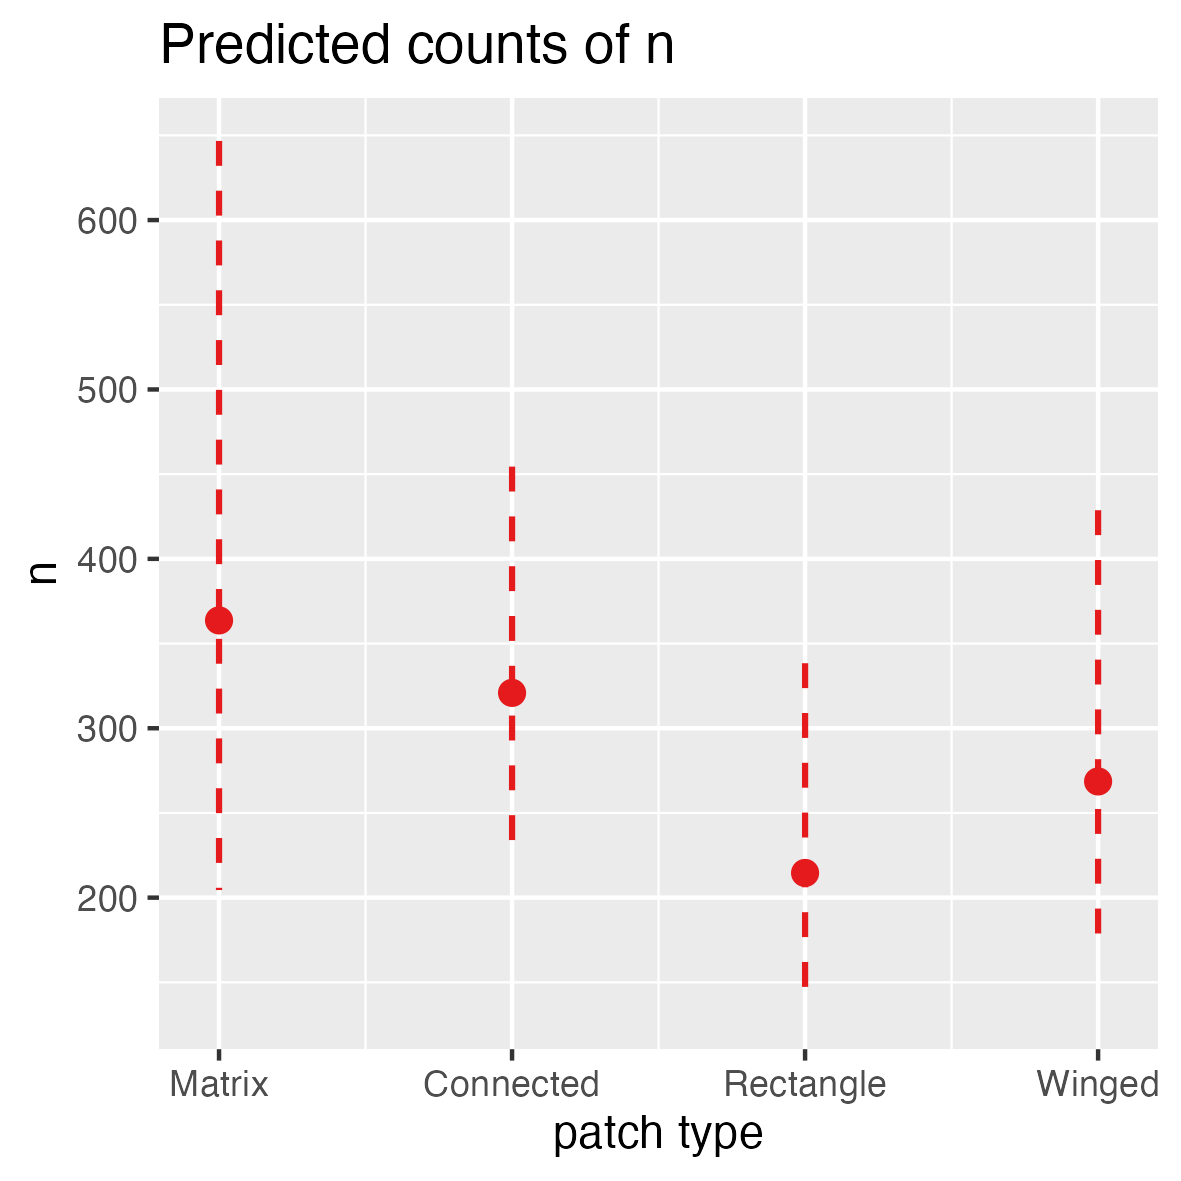
\includegraphics[width=0.7\linewidth,]{images/total_abund} 

}

\caption{Average total dung beetle abundance by patch type with standard deviations as error bars.}\label{fig:patch}
\end{figure}

\newpage

\begin{Shaded}
\begin{Highlighting}[]
\NormalTok{sp\_code\_table}\OtherTok{\textless{}{-}}\FunctionTok{data.frame}\NormalTok{(}\AttributeTok{sp\_code=}\FunctionTok{c}\NormalTok{(}\StringTok{"aaeg"}\NormalTok{, }\StringTok{"cvig"}\NormalTok{, }\StringTok{"dcar"}\NormalTok{, }\StringTok{"open"}\NormalTok{, }\StringTok{"pign"}\NormalTok{, }\StringTok{"alec"}\NormalTok{))}
\NormalTok{species\_names}\OtherTok{\textless{}{-}}\NormalTok{spp\_codes }\SpecialCharTok{\%\textgreater{}\%} 
  \FunctionTok{filter}\NormalTok{(sp\_code}\SpecialCharTok{\%in\%}\NormalTok{sp\_code\_table}\SpecialCharTok{$}\NormalTok{sp\_code) }\SpecialCharTok{\%\textgreater{}\%} 
  \FunctionTok{mutate}\NormalTok{(}\AttributeTok{species=}\FunctionTok{tolower}\NormalTok{(species)) }\SpecialCharTok{\%\textgreater{}\%} 
  \FunctionTok{mutate}\NormalTok{(}\AttributeTok{species=}\FunctionTok{paste}\NormalTok{(}\AttributeTok{species=}\NormalTok{genus,species,}\AttributeTok{sep=}\StringTok{" "}\NormalTok{)) }\SpecialCharTok{\%\textgreater{}\%} 
  \FunctionTok{select}\NormalTok{(sp\_code, species) }\SpecialCharTok{\%\textgreater{}\%} 
\FunctionTok{mutate}\NormalTok{(}\AttributeTok{species=}\FunctionTok{paste}\NormalTok{(sp\_code,species,}\AttributeTok{sep=}\StringTok{": "}\NormalTok{)) }
\NormalTok{species\_names}\OtherTok{\textless{}{-}}\FunctionTok{paste}\NormalTok{(species\_names}\SpecialCharTok{$}\NormalTok{species,}\AttributeTok{collapse=}\StringTok{", "}\NormalTok{)}
\end{Highlighting}
\end{Shaded}

\newpage

\begin{figure}[H]

{\centering 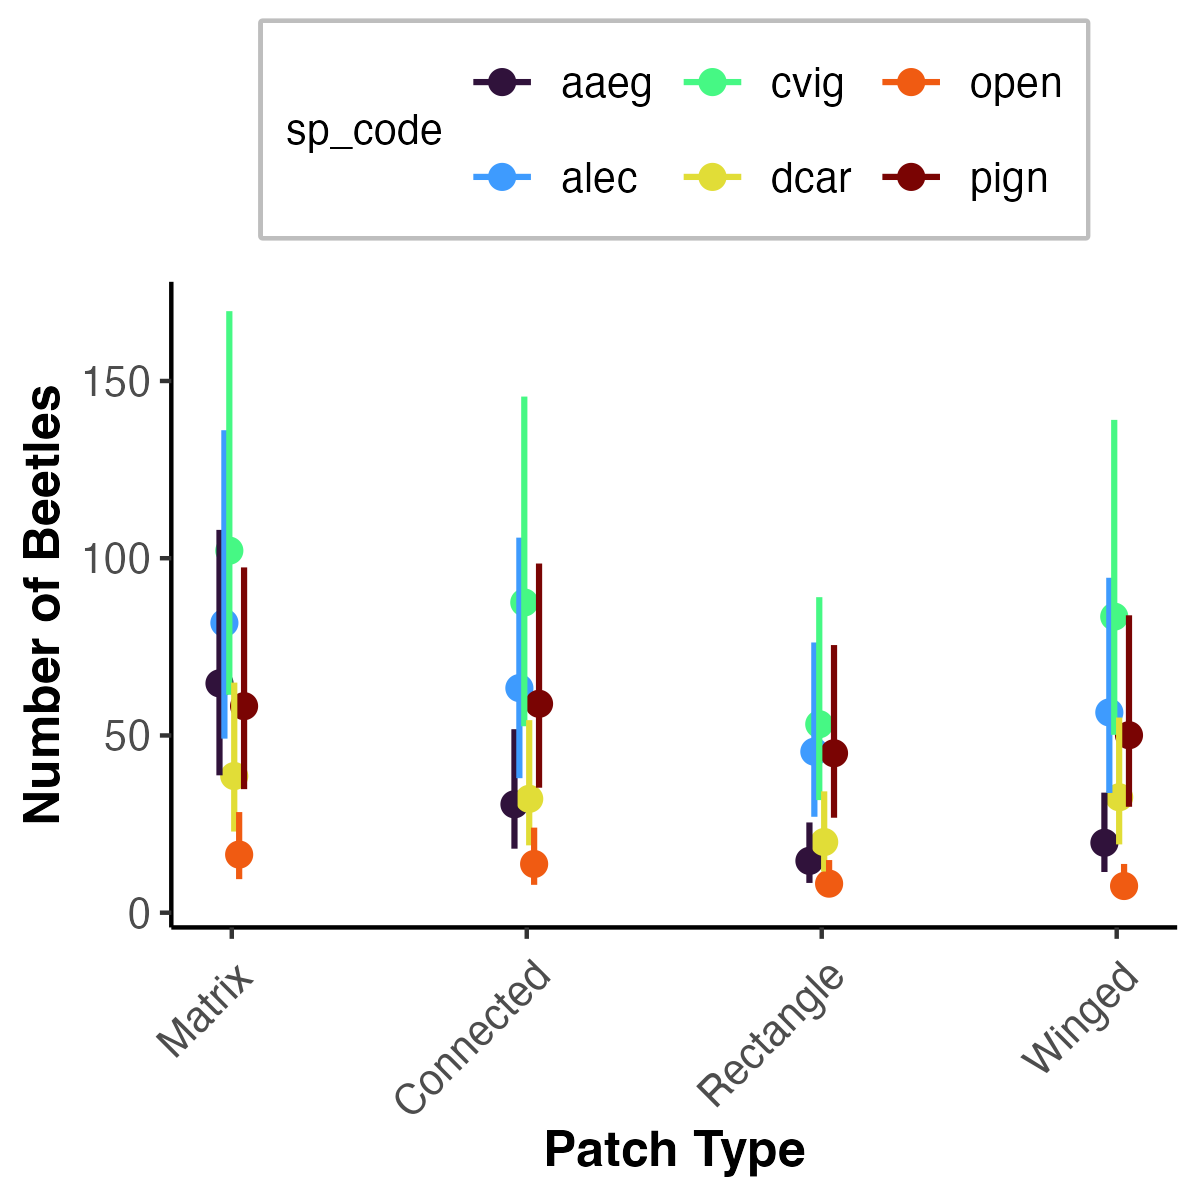
\includegraphics[width=0.7\linewidth,]{images/sp_abund_patch} 

}

\caption{Average abundance of the top 6 most abundant species by patch type. Species codes: alec: Ateuchus lecontei, cvig: Canthon vigilans, dcar: Dichotomius carolinus, open: Onthophagus pennsylvanicus, pign: Phanaeus igneus, aaeg: Aphodius alloblackburneus.}\label{fig:abundance}
\end{figure}

\newpage

\begin{figure}[H]

{\centering 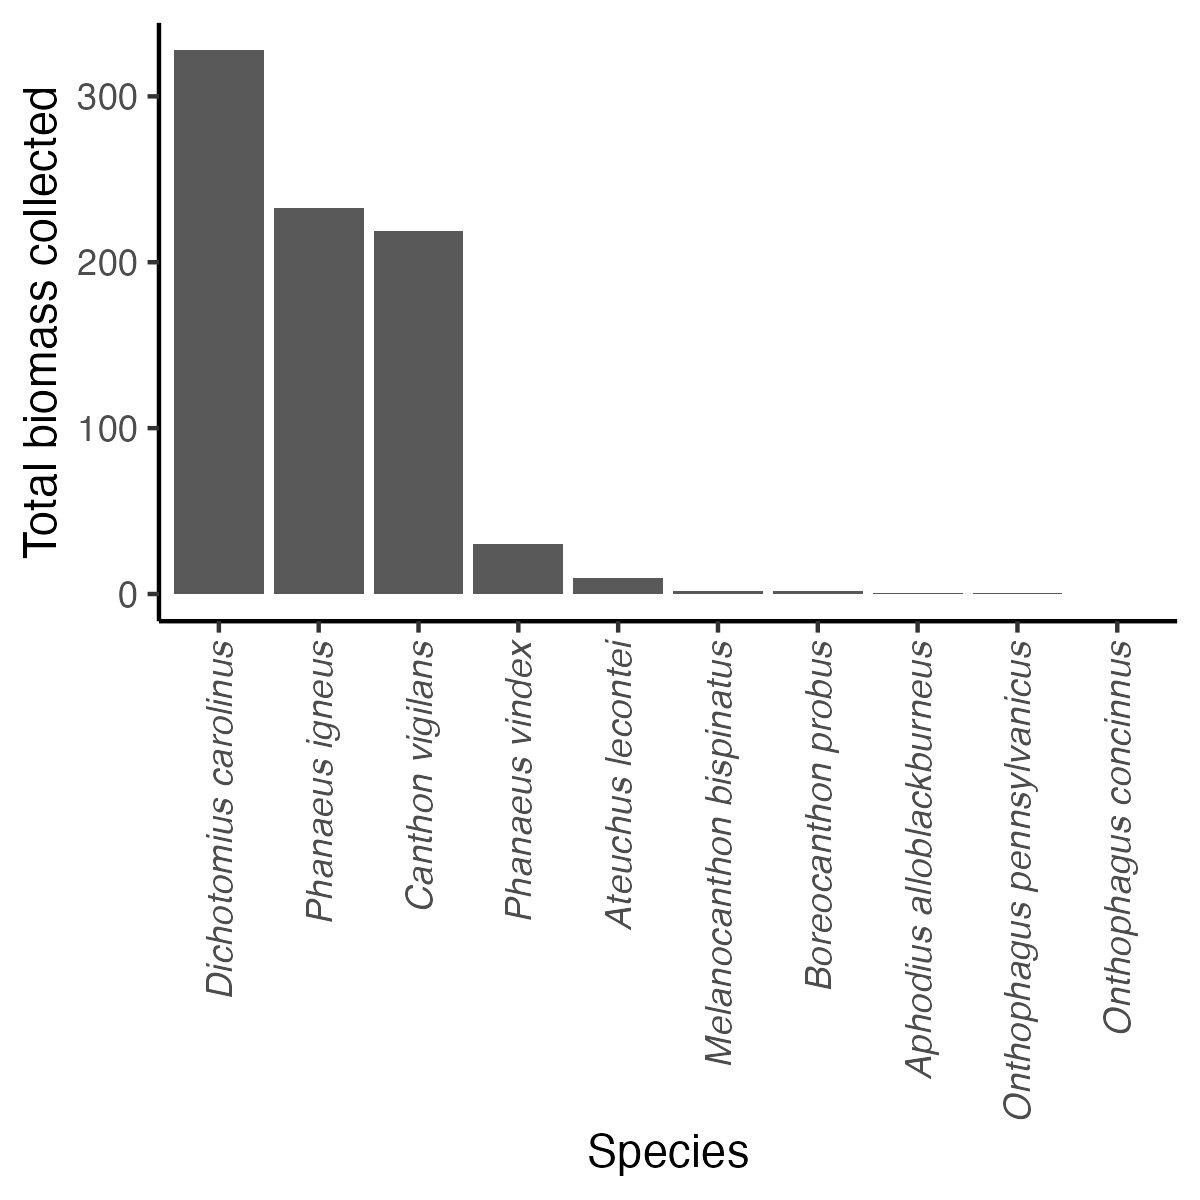
\includegraphics[width=0.7\linewidth,]{images/sp_biomass_plot} 

}

\caption{Total dung beetle biomass collected for each species with sufficient weights.}\label{fig:sp-bmass}
\end{figure}

\newpage

\begin{figure}[H]

{\centering 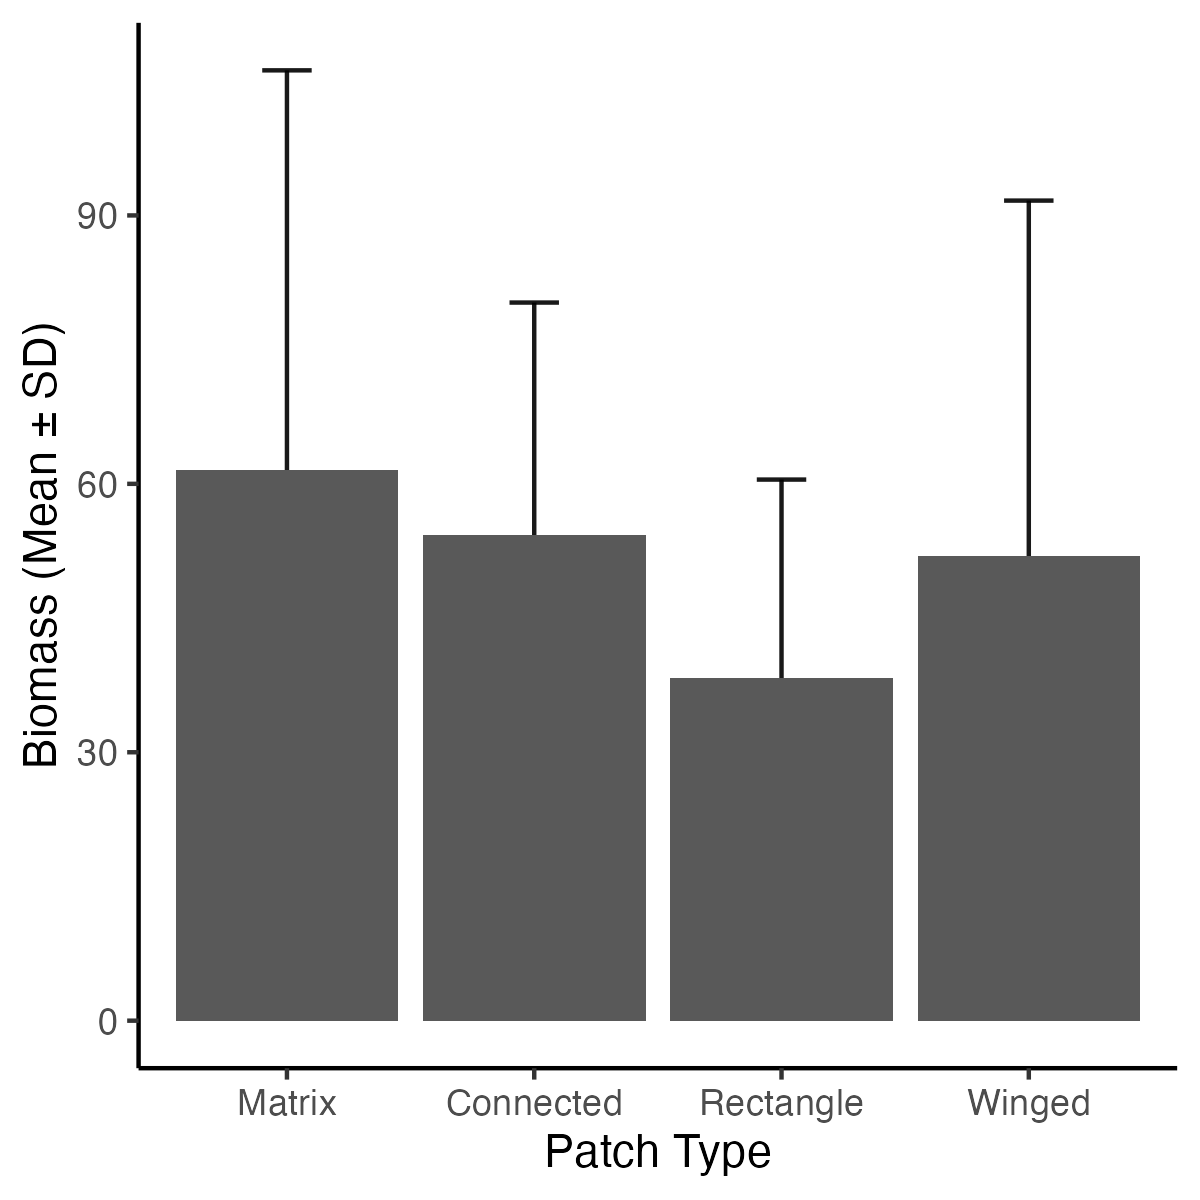
\includegraphics[width=0.7\linewidth,]{images/avg_bmass_patch_plot} 

}

\caption{Average total biomass by patch type with standard deviation as error bars.}\label{fig:patch-bmass}
\end{figure}

\newpage

\begin{figure}[H]

{\centering 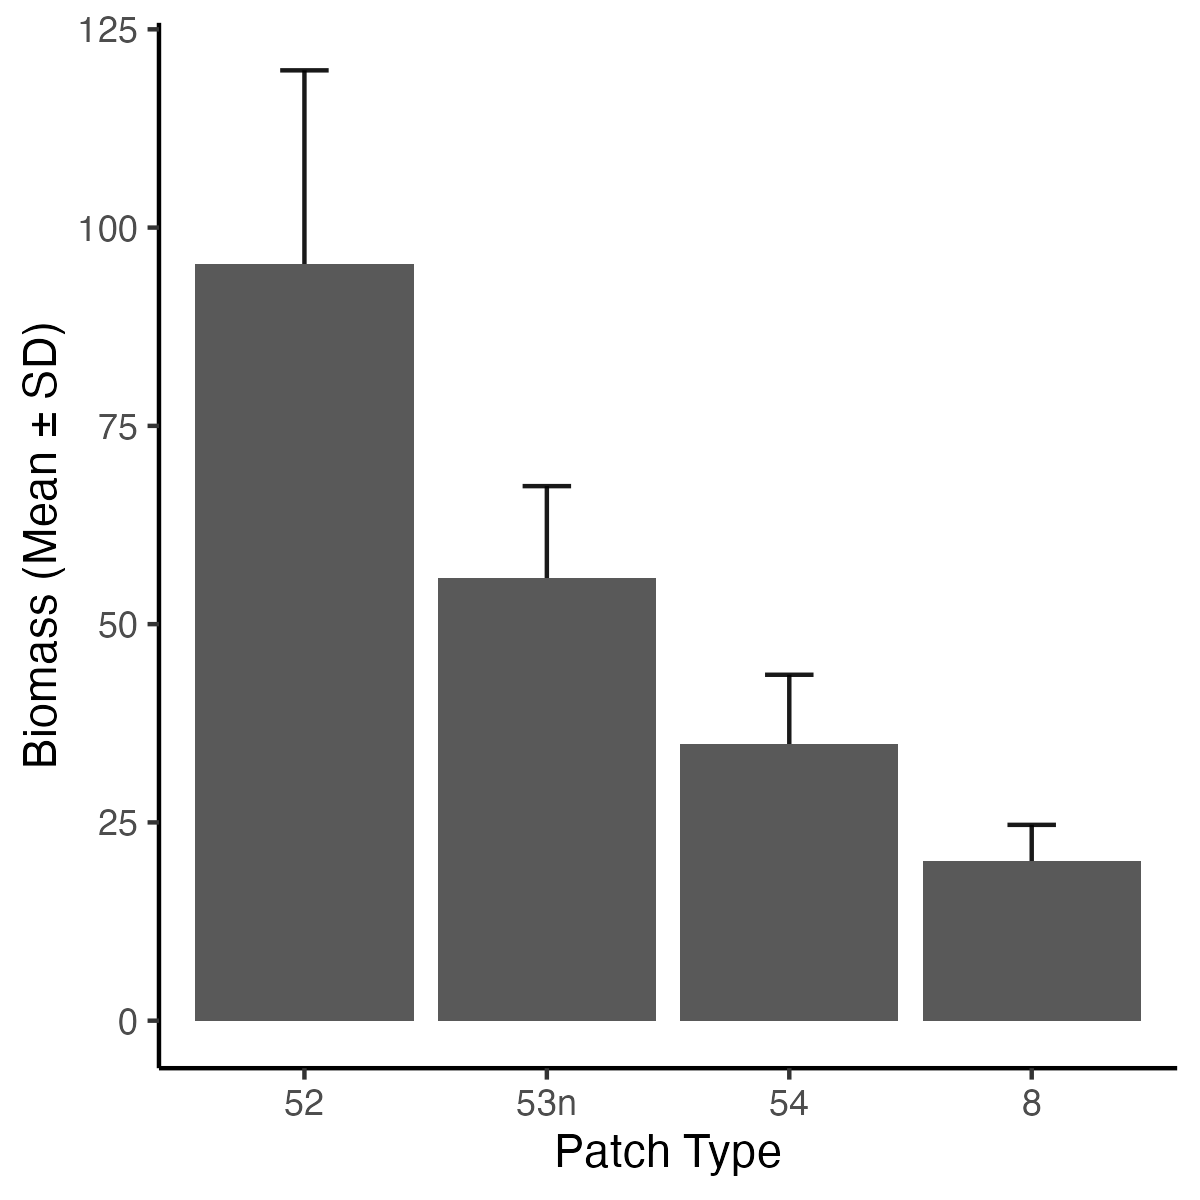
\includegraphics[width=0.7\linewidth,]{images/avg_bmass_block_plot} 

}

\caption{Average total biomass by sampling block with standard deviation as error bars.}\label{fig:block-bmass}
\end{figure}

\newpage

\begin{figure}[H]

{\centering 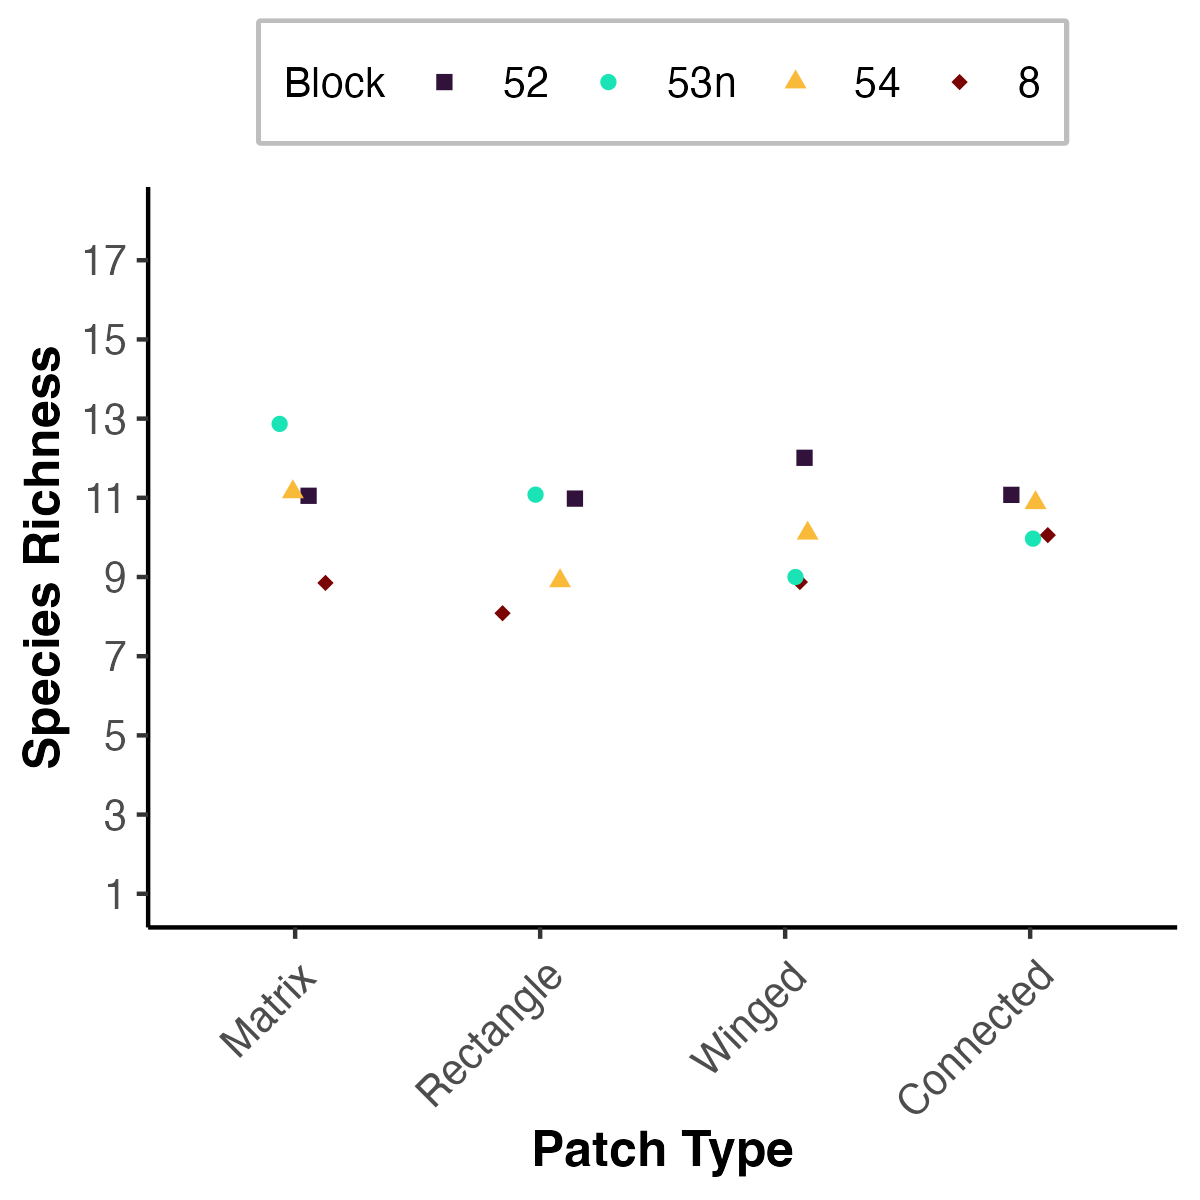
\includegraphics[width=0.7\linewidth,]{images/sp_richness_patches} 

}

\caption{Dung beetle species richness in each patch type. The point shapes indicates the block in which each patch was located.}\label{fig:richness}
\end{figure}

\newpage

\begin{figure}[H]

{\centering 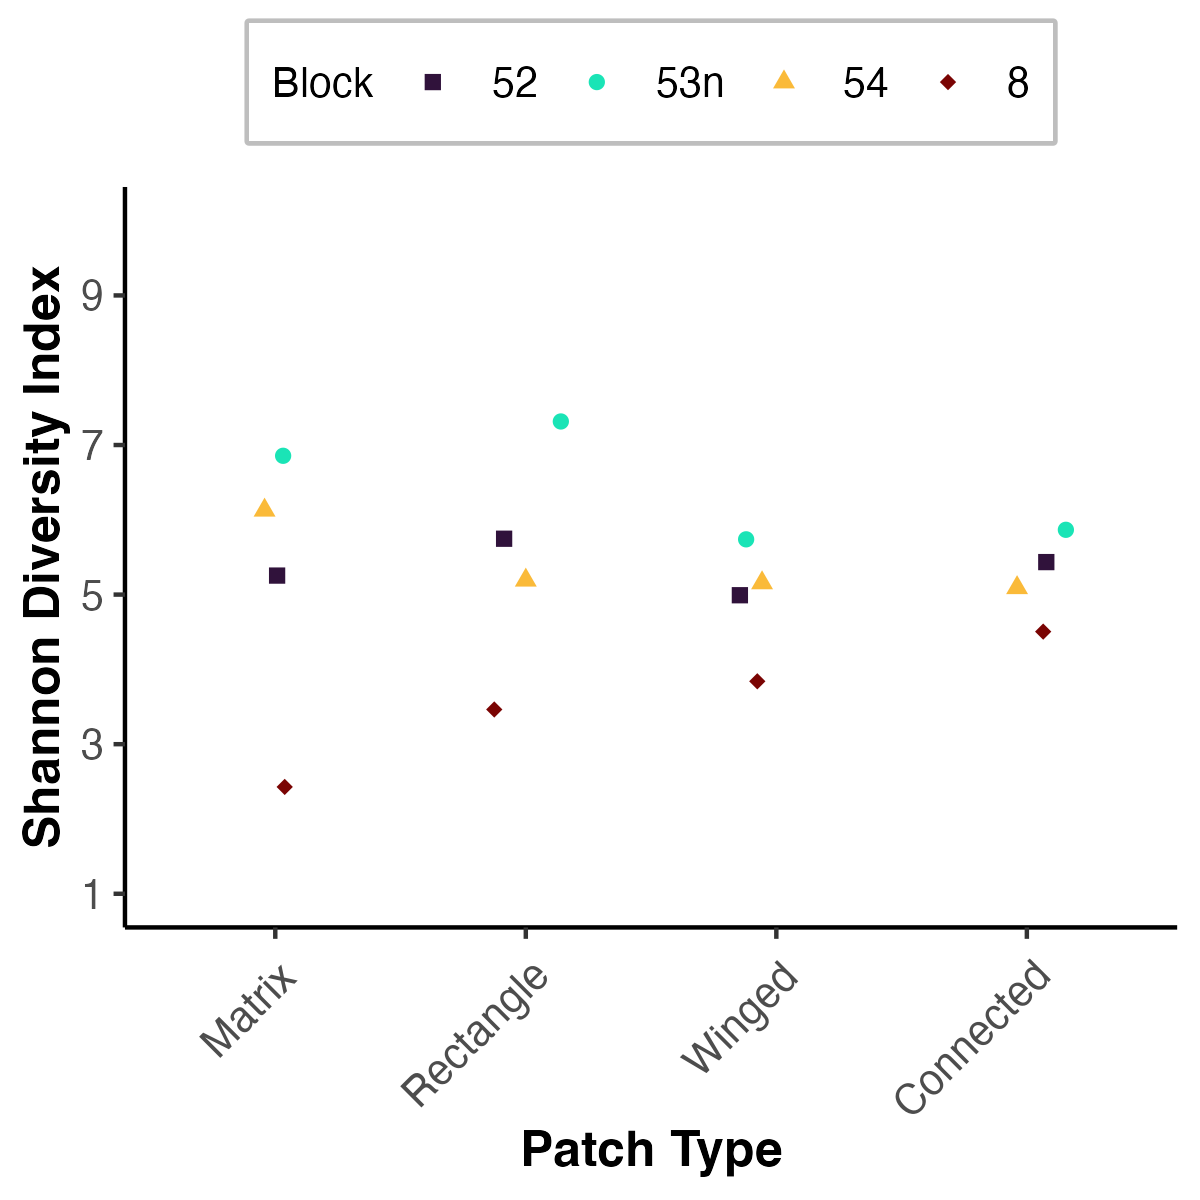
\includegraphics[width=0.7\linewidth,]{images/sp_shannon_patches} 

}

\caption{Dung beetle Shannon diversity by patch type.}\label{fig:shannon}
\end{figure}

\newpage

\begin{figure}[H]

{\centering 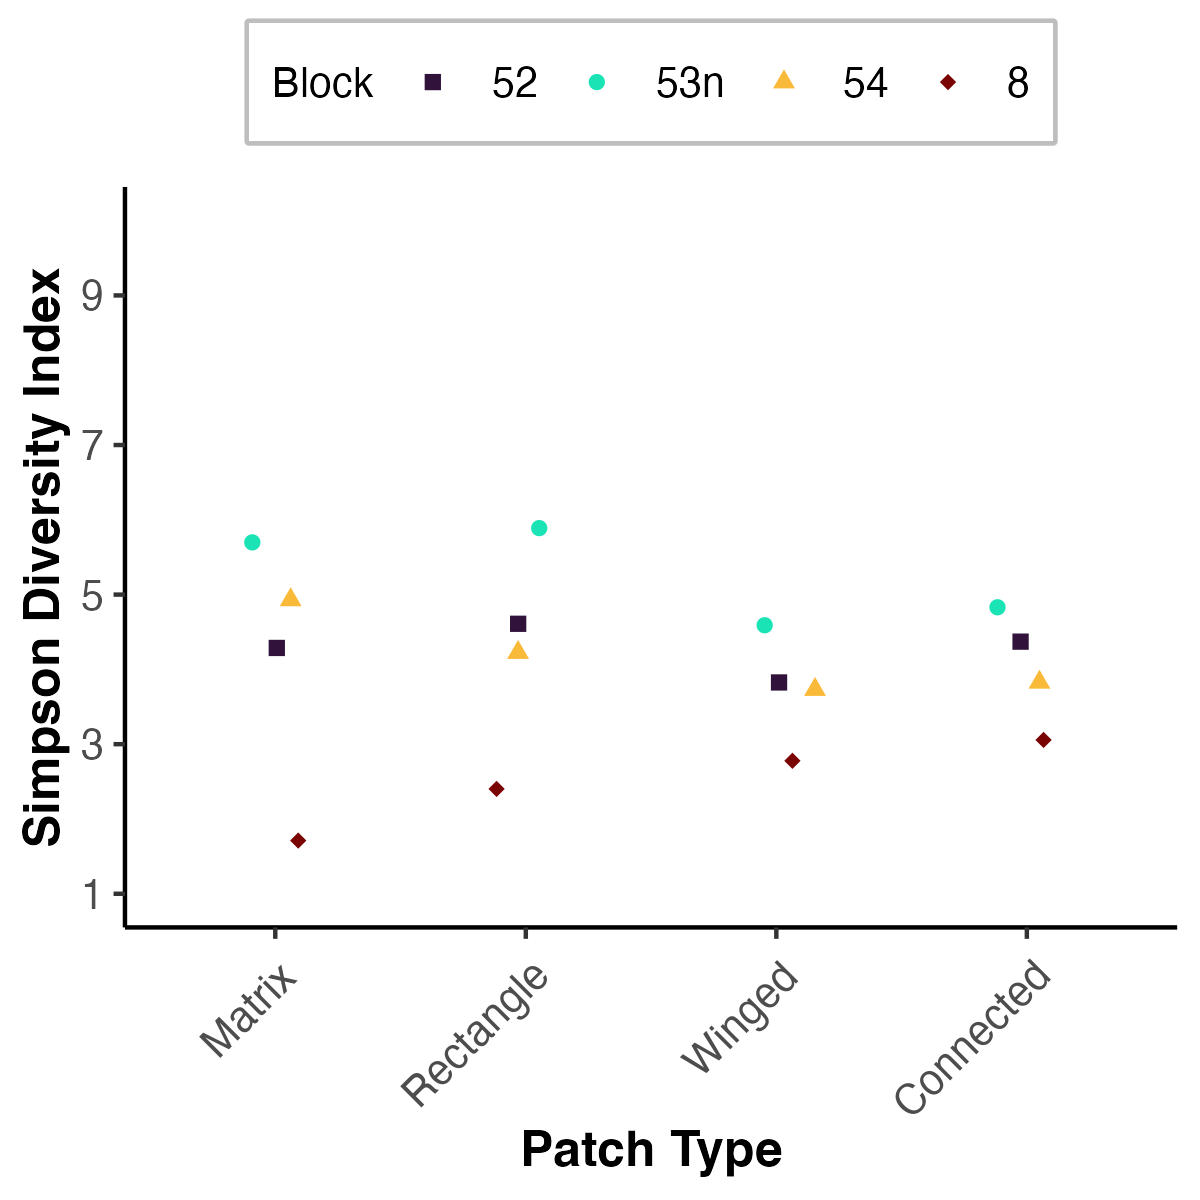
\includegraphics[width=0.7\linewidth,]{images/sp_simpson_patches} 

}

\caption{Dung beetle Simpson's index by patch type.}\label{fig:simpson}
\end{figure}

\newpage

\begin{center}
\end{center}


\end{document}
